\documentclass[aspectratio=169,11.5pt]{beamer}


% Cargar la plantilla
\input{~/Dropbox/Latex/TemplateSlides/template-slide.tex}


% ==========================
% PERSONALIZACIÓN POR CLASE
% ==========================
\renewcommand{\CourseName}{Diseño Web 1}
\renewcommand{\CourseCode}{ADSO-CTMA}
\renewcommand{\Faculty}{}
\renewcommand{\Institution}{Servicio Nacional de Aprendizaje SENA}
\renewcommand{\Instructor}{Deimer Miranda Montoya, MSc.(c).}
\renewcommand{\Email}{damiranda@sena.edu.co}

\newcommand{\ok}{\textcolor{green}{\faCheck}}
\newcommand{\fail}{\textcolor{red}{\faTimes}}

% Meta
\title{\CourseName}
\author{\Instructor}
\date{\today}

\begin{document}

    % Portada
    \TitleSlide

    % Normas
    \NormasSlide


    %==========================================================================================================================
    % ===================== Reflexión ==================
    %==========================================================================================================================
    \begin{frame}{Reflexión inicial}
        \centering
        \textbf{\large
            "La única persona que puede decirte ‘no puedes lograrlo’ eres tú misma, y no debes escucharla"\\Jessica Ennis.}

        \vspace{0.4cm}
        \smartimage[4cm]{Template/person.png}
    \end{frame}

    % (Opcional) Agenda
    %\AgendaSlide


    %=====================================================================================================================
    % ===================== Inicio ==================
    %=====================================================================================================================

    % =========================================================
    % CLASE 6 - BLOQUE 1
    % FLEXBOX: FUNDAMENTOS, CONTENEDOR Y EJES
    % =========================================================

    \section{Clase 6}

    \SectionSlide
    {Flexbox}
    {Distribuir y alinear elementos dentro de un contenedor}

    % ---------------------------------------------------------
    \begin{frame}{Propósito de la clase}
        Al finalizar la clase, el aprendiz estará en capacidad de:

        \begin{itemize}
            \item Explicar qué es Flexbox y para qué se utiliza.
            \item Diferenciar contenedor flex y elementos flex.
            \item Comprender el eje principal y el eje transversal.
            \item Aplicar \texttt{display: flex}.
            \item Utilizar \texttt{flex-direction}.
            \item Distribuir elementos con \texttt{justify-content}.
            \item Alinear elementos con \texttt{align-items}.
            \item Separar elementos mediante \texttt{gap}.
        \end{itemize}

        \begin{block}{Pregunta orientadora}
            ¿Cómo podemos organizar varios elementos sin moverlos
            manualmente uno por uno?
        \end{block}
    \end{frame}

    % ---------------------------------------------------------
    \begin{frame}{¿Por qué necesitamos Flexbox?}
        Hasta ahora hemos trabajado elementos individuales:

        \begin{itemize}
            \item Tamaño de una caja.
            \item Espacio interno y externo.
            \item Bordes.
            \item Posicionamiento puntual.
        \end{itemize}

        Pero muchas interfaces necesitan organizar varios elementos:

        \begin{itemize}
            \item Menús.
            \item Tarjetas.
            \item Botones.
            \item Galerías.
            \item Secciones de contenido.
        \end{itemize}

        \begin{block}{Idea clave}
            Flexbox permite distribuir elementos dentro de un contenedor
            de forma más flexible y controlada.
        \end{block}
    \end{frame}

    % ---------------------------------------------------------
    \begin{frame}{Problema inicial}
        Supongamos tres cajas dentro de un contenedor.

        Sin Flexbox, normalmente aparecen una debajo de otra
        si son elementos de bloque.

        \begin{center}
            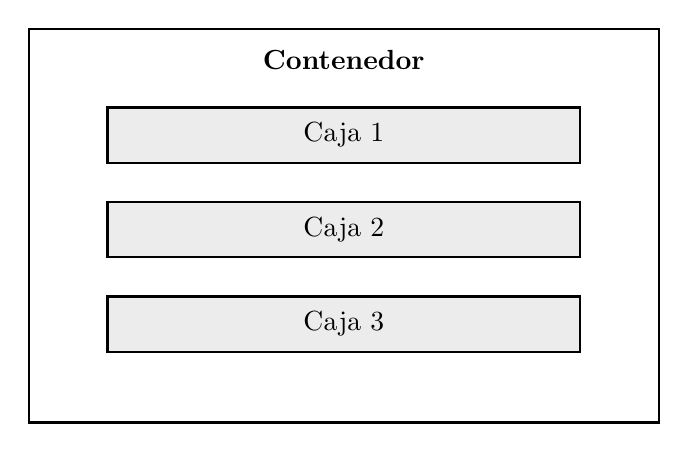
\begin{tikzpicture}
                \draw[thick] (0,0) rectangle (8,5);
                \node at (4,4.6) {\textbf{Contenedor}};

                \draw[fill=gray!15, thick] (1,3.3) rectangle (7,4);
                \node at (4,3.65) {Caja 1};

                \draw[fill=gray!15, thick] (1,2.1) rectangle (7,2.8);
                \node at (4,2.45) {Caja 2};

                \draw[fill=gray!15, thick] (1,0.9) rectangle (7,1.6);
                \node at (4,1.25) {Caja 3};
            \end{tikzpicture}
        \end{center}
    \end{frame}

    % ---------------------------------------------------------
    \begin{frame}[fragile]{HTML base del ejemplo}
        Para los ejemplos usaremos una estructura pequeña:

        \begin{htmlcodedark}
            <div class="contenedor">
            <div class="caja">Caja 1</div>
            <div class="caja">Caja 2</div>
            <div class="caja">Caja 3</div>
            </div>
        \end{htmlcodedark}

        \begin{block}{Observación}
            El elemento con clase \texttt{contenedor}
            agrupa las tres cajas.
        \end{block}
    \end{frame}

    % ---------------------------------------------------------
    \begin{frame}[fragile]{CSS base del ejemplo}
        Antes de usar Flexbox, aplicamos estilos simples:

        \begin{csscodedark}
            .contenedor {
                border: 2px solid black;
                padding: 10px;
            }

            .caja {
                border: 1px solid gray;
                padding: 15px;
                margin: 5px;
            }
        \end{csscodedark}

        \begin{block}{Importante}
            Aquí todavía no hay Flexbox.
            Solo estamos haciendo visibles las cajas.
        \end{block}
    \end{frame}

    % =========================================================
    % ¿QUÉ ES FLEXBOX?
    % =========================================================

    \section{Fundamentos de Flexbox}

    \SectionSlide
    {Fundamentos de Flexbox}
    {Contenedor flex y elementos flex}

    % ---------------------------------------------------------
    \begin{frame}{¿Qué es Flexbox?}
        Flexbox es un modelo de diseño de CSS pensado
        para organizar elementos dentro de un contenedor.

        Su nombre proviene de:

        \begin{center}
            \Large
            \textbf{Flexible Box Layout}
        \end{center}

        En español:

        \begin{center}
            \large
            \textbf{Modelo de cajas flexibles}
        \end{center}

        \begin{block}{Idea clave}
            Flexbox no se aplica a una caja aislada,
            sino a la relación entre un contenedor
            y sus elementos internos.
        \end{block}
    \end{frame}

    % ---------------------------------------------------------
    \begin{frame}{Contenedor flex y elementos flex}
        Flexbox trabaja con dos conceptos principales:

        \begin{description}
            \item[Contenedor flex:]
            elemento padre al que se le aplica
            \texttt{display: flex}.

            \item[Elementos flex:]
            elementos hijos directos del contenedor flex.
        \end{description}

        \begin{center}
            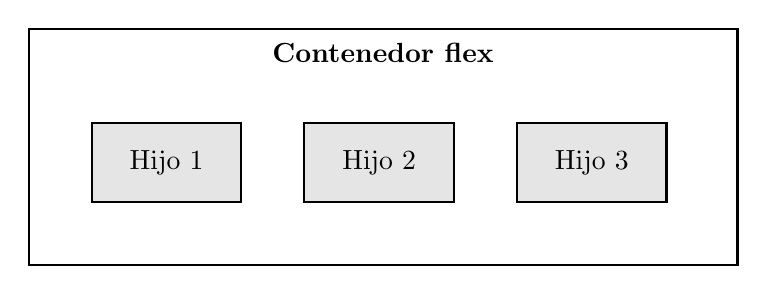
\begin{tikzpicture}
                \draw[thick] (0,0) rectangle (9,3);
                \node at (4.5,2.7) {\textbf{Contenedor flex}};

                \draw[fill=gray!20, thick] (0.8,0.8) rectangle (2.7,1.8);
                \node at (1.75,1.3) {Hijo 1};

                \draw[fill=gray!20, thick] (3.5,0.8) rectangle (5.4,1.8);
                \node at (4.45,1.3) {Hijo 2};

                \draw[fill=gray!20, thick] (6.2,0.8) rectangle (8.1,1.8);
                \node at (7.15,1.3) {Hijo 3};
            \end{tikzpicture}
        \end{center}
    \end{frame}

    % ---------------------------------------------------------
    \begin{frame}[fragile]{Activar Flexbox}
        Flexbox se activa en el contenedor:

        \begin{csscodedark}
            .contenedor {
                display: flex;
            }
        \end{csscodedark}

        \begin{block}{Efecto}
            Los hijos directos de \texttt{.contenedor}
            pasan a comportarse como elementos flex.
        \end{block}

        \begin{alertblock}{Importante}
            \texttt{display: flex} se escribe en el padre,
            no en cada hijo.
        \end{alertblock}
    \end{frame}

    % ---------------------------------------------------------
    \begin{frame}{Antes y después de display flex}
        \begin{center}
            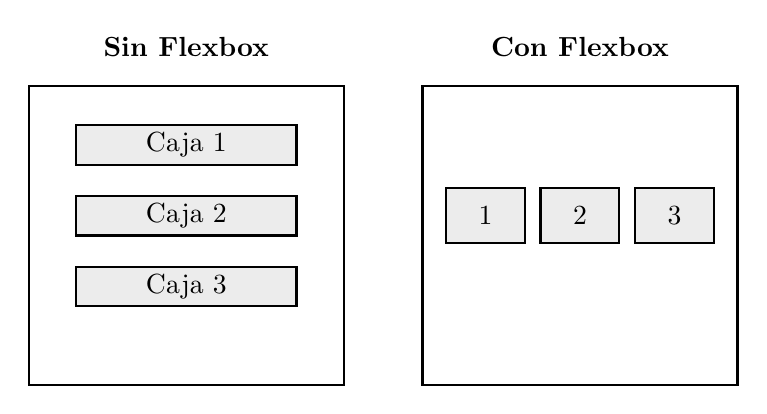
\begin{tikzpicture}
                \node at (2,4.5) {\textbf{Sin Flexbox}};
                \draw[thick] (0,0.2) rectangle (4,4);

                \draw[fill=gray!15, thick] (0.6,3) rectangle (3.4,3.5);
                \node at (2,3.25) {Caja 1};

                \draw[fill=gray!15, thick] (0.6,2.1) rectangle (3.4,2.6);
                \node at (2,2.35) {Caja 2};

                \draw[fill=gray!15, thick] (0.6,1.2) rectangle (3.4,1.7);
                \node at (2,1.45) {Caja 3};

                \node at (7,4.5) {\textbf{Con Flexbox}};
                \draw[thick] (5,0.2) rectangle (9,4);

                \draw[fill=gray!15, thick] (5.3,2) rectangle (6.3,2.7);
                \node at (5.8,2.35) {1};

                \draw[fill=gray!15, thick] (6.5,2) rectangle (7.5,2.7);
                \node at (7,2.35) {2};

                \draw[fill=gray!15, thick] (7.7,2) rectangle (8.7,2.7);
                \node at (8.2,2.35) {3};
            \end{tikzpicture}
        \end{center}
    \end{frame}

    % ---------------------------------------------------------
    \begin{frame}[fragile]{Ejemplo mínimo completo}
        HTML:

        \begin{htmlcodedark}
            <div class="contenedor">
            <div class="caja">1</div>
            <div class="caja">2</div>
            <div class="caja">3</div>
            </div>
        \end{htmlcodedark}

        CSS:

        \begin{csscodedark}
            .contenedor {
                display: flex;
            }
        \end{csscodedark}

        \begin{block}{Resultado}
            Las cajas hijas se organizan inicialmente
            en una fila.
        \end{block}
    \end{frame}

    % =========================================================
    % EJES DE FLEXBOX
    % =========================================================

    \section{Ejes de Flexbox}

    \SectionSlide
    {Ejes de Flexbox}
    {Eje principal y eje transversal}

    % ---------------------------------------------------------
    \begin{frame}{¿Por qué hablar de ejes?}
        Flexbox organiza los elementos siguiendo dos ejes:

        \begin{itemize}
            \item Eje principal.
            \item Eje transversal.
        \end{itemize}

        \begin{block}{Idea clave}
            Muchas propiedades de Flexbox no significan
            ``horizontal'' o ``vertical'' de forma fija.

            Dependen del eje principal definido.
        \end{block}
    \end{frame}

    % ---------------------------------------------------------
    \begin{frame}{Eje principal y eje transversal}
        \begin{center}
            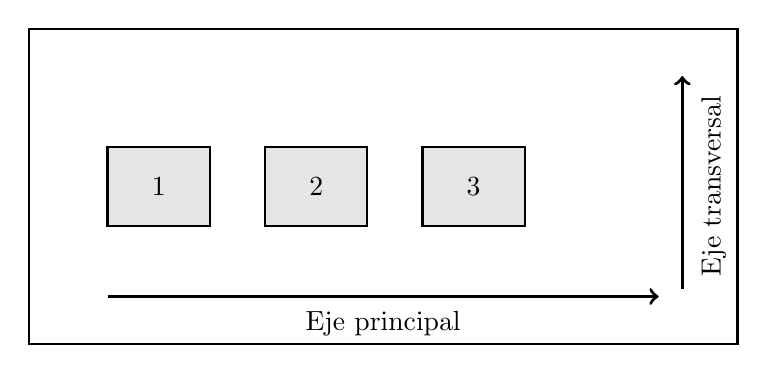
\begin{tikzpicture}
                \draw[thick] (0,0) rectangle (9,4);

                \draw[fill=gray!20, thick] (1,1.5) rectangle (2.3,2.5);
                \node at (1.65,2) {1};

                \draw[fill=gray!20, thick] (3,1.5) rectangle (4.3,2.5);
                \node at (3.65,2) {2};

                \draw[fill=gray!20, thick] (5,1.5) rectangle (6.3,2.5);
                \node at (5.65,2) {3};

                \draw[->, very thick] (1,0.6) -- (8,0.6);
                \node at (4.5,0.25) {Eje principal};

                \draw[->, very thick] (8.3,0.7) -- (8.3,3.4);
                \node[rotate=90] at (8.7,2) {Eje transversal};
            \end{tikzpicture}
        \end{center}

        \begin{block}{Caso inicial}
            Por defecto, Flexbox organiza los elementos
            en dirección horizontal.
        \end{block}
    \end{frame}

    % ---------------------------------------------------------
    \begin{frame}{Eje principal}
        El eje principal indica la dirección en la que
        se distribuyen los elementos flex.

        Por defecto:

        \begin{center}
            \Large
            izquierda $\rightarrow$ derecha
        \end{center}

        En ese caso, los elementos se organizan en una fila.

        \begin{block}{Propiedad relacionada}
            La propiedad que controla el eje principal es:

            \texttt{flex-direction}
        \end{block}
    \end{frame}

    % ---------------------------------------------------------
    \begin{frame}{Eje transversal}
        El eje transversal cruza al eje principal.

        Si el eje principal es horizontal,
        el eje transversal será vertical.

        \begin{center}
            \Large
            eje principal: horizontal

            \vspace{0.3cm}

            eje transversal: vertical
        \end{center}

        \begin{block}{Idea}
            Algunas propiedades alinean sobre el eje principal
            y otras sobre el eje transversal.
        \end{block}
    \end{frame}

    % =========================================================
    % FLEX-DIRECTION
    % =========================================================

    \section{flex-direction}

    \SectionSlide
    {flex-direction}
    {Definir la dirección del eje principal}

    % ---------------------------------------------------------
    \begin{frame}{¿Qué hace flex-direction?}
        La propiedad \texttt{flex-direction}
        define la dirección del eje principal.

        Valores principales:

        \begin{itemize}
            \item \texttt{row}
            \item \texttt{row-reverse}
            \item \texttt{column}
            \item \texttt{column-reverse}
        \end{itemize}

        \begin{block}{Sintaxis}
            \texttt{flex-direction: valor;}
        \end{block}
    \end{frame}

    % ---------------------------------------------------------
    \begin{frame}[fragile]{flex-direction: row}
        Es el valor predeterminado.

        \begin{csscodedark}
            .contenedor {
                display: flex;
                flex-direction: row;
            }
        \end{csscodedark}

        \begin{center}
            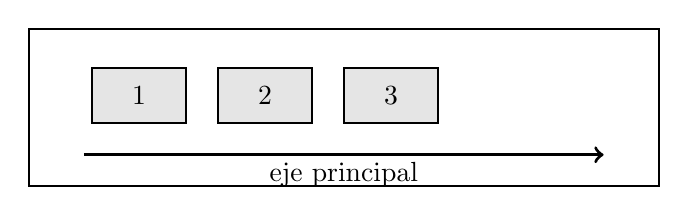
\begin{tikzpicture}
                \draw[thick] (0,0) rectangle (8,2);
                \draw[->, very thick] (0.7,0.4) -- (7.3,0.4);
                \node at (4,0.15) {eje principal};

                \draw[fill=gray!20, thick] (0.8,0.8) rectangle (2,1.5);
                \node at (1.4,1.15) {1};

                \draw[fill=gray!20, thick] (2.4,0.8) rectangle (3.6,1.5);
                \node at (3,1.15) {2};

                \draw[fill=gray!20, thick] (4,0.8) rectangle (5.2,1.5);
                \node at (4.6,1.15) {3};
            \end{tikzpicture}
        \end{center}
    \end{frame}

    % ---------------------------------------------------------
    \begin{frame}[fragile]{flex-direction: row-reverse}
        Invierte la dirección horizontal.

        \begin{csscodedark}
            .contenedor {
                display: flex;
                flex-direction: row-reverse;
            }
        \end{csscodedark}

        \begin{center}
            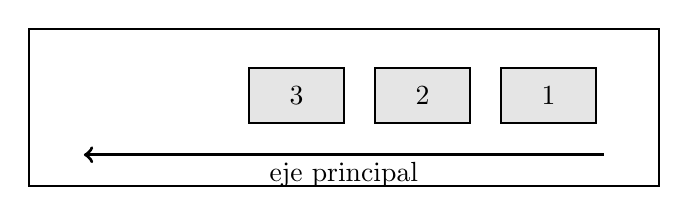
\begin{tikzpicture}
                \draw[thick] (0,0) rectangle (8,2);
                \draw[->, very thick] (7.3,0.4) -- (0.7,0.4);
                \node at (4,0.15) {eje principal};

                \draw[fill=gray!20, thick] (6,0.8) rectangle (7.2,1.5);
                \node at (6.6,1.15) {1};

                \draw[fill=gray!20, thick] (4.4,0.8) rectangle (5.6,1.5);
                \node at (5,1.15) {2};

                \draw[fill=gray!20, thick] (2.8,0.8) rectangle (4,1.5);
                \node at (3.4,1.15) {3};
            \end{tikzpicture}
        \end{center}
    \end{frame}

    % ---------------------------------------------------------
    \begin{frame}[fragile]{flex-direction: column}
        Cambia el eje principal a vertical.

        \begin{csscodedark}
            .contenedor {
                display: flex;
                flex-direction: column;
            }
        \end{csscodedark}

        \begin{center}
            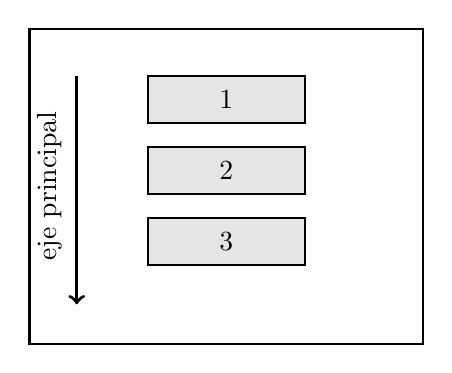
\begin{tikzpicture}
                \draw[thick] (0,0) rectangle (5,4);

                \draw[->, very thick] (0.6,3.4) -- (0.6,0.5);
                \node[rotate=90] at (0.25,2) {eje principal};

                \draw[fill=gray!20, thick] (1.5,2.8) rectangle (3.5,3.4);
                \node at (2.5,3.1) {1};

                \draw[fill=gray!20, thick] (1.5,1.9) rectangle (3.5,2.5);
                \node at (2.5,2.2) {2};

                \draw[fill=gray!20, thick] (1.5,1) rectangle (3.5,1.6);
                \node at (2.5,1.3) {3};
            \end{tikzpicture}
        \end{center}
    \end{frame}

    % ---------------------------------------------------------
    \begin{frame}[fragile]{flex-direction: column-reverse}
        Invierte la dirección vertical.

        \begin{csscodedark}
            .contenedor {
                display: flex;
                flex-direction: column-reverse;
            }
        \end{csscodedark}

        \begin{block}{Resultado}
            El eje principal es vertical,
            pero el orden visual se presenta
            desde abajo hacia arriba.
        \end{block}
    \end{frame}

    % ---------------------------------------------------------
    \begin{frame}{Resumen de flex-direction}
        \begin{center}
            \small
            \begin{tabular}{p{3cm}p{5.8cm}}
                \toprule
                \textbf{Valor} & \textbf{Comportamiento} \\
                \midrule
                \texttt{row} & organiza de izquierda a derecha. \\
                \texttt{row-reverse} & organiza de derecha a izquierda. \\
                \texttt{column} & organiza de arriba hacia abajo. \\
                \texttt{column-reverse} & organiza de abajo hacia arriba. \\
                \bottomrule
            \end{tabular}
        \end{center}

        \begin{alertblock}{Importante}
            Cambiar \texttt{flex-direction} también cambia
            la interpretación de otras propiedades.
        \end{alertblock}
    \end{frame}

    % =========================================================
    % CLASE 6 - BLOQUE 2
    % JUSTIFY-CONTENT, ALIGN-ITEMS, GAP Y FLEX-WRAP
    % =========================================================

    % =========================================================
    % JUSTIFY-CONTENT
    % =========================================================

    \section{justify-content}

    \SectionSlide
    {justify-content}
    {Distribuir elementos sobre el eje principal}

    % ---------------------------------------------------------
    \begin{frame}{¿Qué hace justify-content?}
        La propiedad \texttt{justify-content}
        controla la distribución de los elementos
        sobre el \textbf{eje principal}.

        \begin{block}{Idea clave}
            Para interpretar correctamente
            \texttt{justify-content},
            primero debemos identificar
            cuál es el eje principal.
        \end{block}

        Por defecto:

        \begin{center}
            \texttt{flex-direction: row;}
        \end{center}

        Por lo tanto, el eje principal es horizontal.
    \end{frame}

    % ---------------------------------------------------------
    \begin{frame}[fragile]{HTML de referencia}
        Continuaremos utilizando:

        \begin{htmlcodedark}
            <div class="contenedor">
            <div class="caja">1</div>
            <div class="caja">2</div>
            <div class="caja">3</div>
            </div>
        \end{htmlcodedark}

        CSS inicial:

        \begin{csscodedark}
            .contenedor {
                display: flex;
            }
        \end{csscodedark}

        Solo modificaremos una propiedad
        en cada ejemplo.
    \end{frame}

    % ---------------------------------------------------------
    \begin{frame}{Valores principales de justify-content}
        En esta clase trabajaremos con:

        \begin{itemize}
            \item \texttt{flex-start}
            \item \texttt{center}
            \item \texttt{flex-end}
            \item \texttt{space-between}
            \item \texttt{space-around}
            \item \texttt{space-evenly}
        \end{itemize}

        \begin{block}{Sintaxis}
            \texttt{justify-content: valor;}
        \end{block}
    \end{frame}

    % ---------------------------------------------------------
    \begin{frame}[fragile]{justify-content: flex-start}
        Es el comportamiento inicial.

        \begin{csscodedark}
            .contenedor {
                display: flex;
                justify-content: flex-start;
            }
        \end{csscodedark}

        \begin{center}
            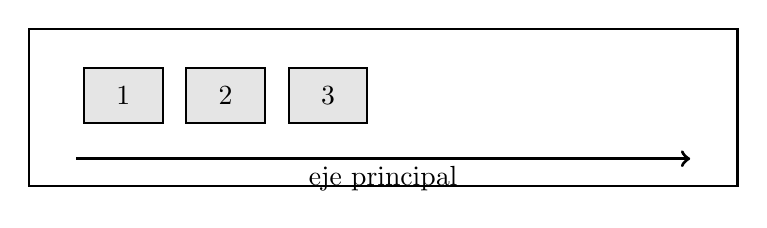
\begin{tikzpicture}
                \draw[thick] (0,0) rectangle (9,2);

                \draw[->, very thick] (0.6,0.35) -- (8.4,0.35);
                \node at (4.5,0.1) {eje principal};

                \foreach \x/\n in {0.7/1,2.0/2,3.3/3}{
                    \draw[fill=gray!20, thick]
                    (\x,0.8) rectangle ++(1,0.7);
                    \node at (\x+0.5,1.15) {\n};
                }
            \end{tikzpicture}
        \end{center}

        Los elementos se ubican al inicio del eje principal.
    \end{frame}

    % ---------------------------------------------------------
    \begin{frame}[fragile]{justify-content: center}
        Cambiamos solamente el valor:

        \begin{csscodedark}
            .contenedor {
                display: flex;
                justify-content: center;
            }
        \end{csscodedark}

        \begin{center}
            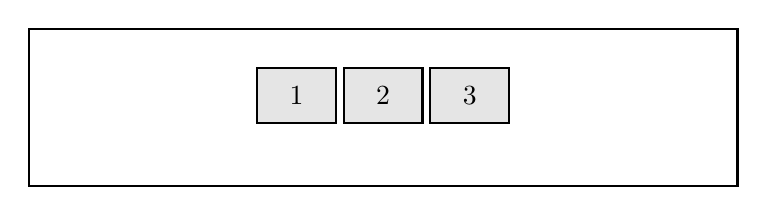
\begin{tikzpicture}
                \draw[thick] (0,0) rectangle (9,2);

                \foreach \x/\n in {2.9/1,4.0/2,5.1/3}{
                    \draw[fill=gray!20, thick]
                    (\x,0.8) rectangle ++(1,0.7);
                    \node at (\x+0.5,1.15) {\n};
                }
            \end{tikzpicture}
        \end{center}

        \begin{block}{Resultado}
            El grupo de elementos se ubica
            en el centro del eje principal.
        \end{block}
    \end{frame}

    % ---------------------------------------------------------
    \begin{frame}[fragile]{justify-content: flex-end}
        \begin{csscodedark}
            .contenedor {
                display: flex;
                justify-content: flex-end;
            }
        \end{csscodedark}

        \begin{center}
            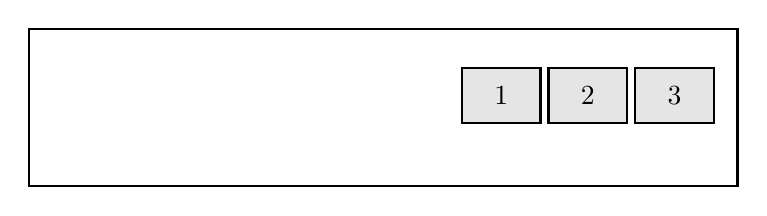
\begin{tikzpicture}
                \draw[thick] (0,0) rectangle (9,2);

                \foreach \x/\n in {5.5/1,6.6/2,7.7/3}{
                    \draw[fill=gray!20, thick]
                    (\x,0.8) rectangle ++(1,0.7);
                    \node at (\x+0.5,1.15) {\n};
                }
            \end{tikzpicture}
        \end{center}

        Los elementos se ubican al final
        del eje principal.
    \end{frame}

    % ---------------------------------------------------------
    \begin{frame}[fragile]{justify-content: space-between}
        \begin{csscodedark}
            .contenedor {
                display: flex;
                justify-content: space-between;
            }
        \end{csscodedark}

        \begin{center}
            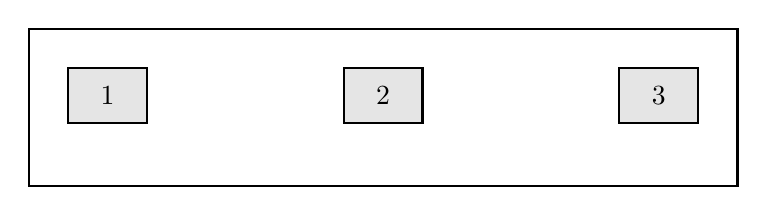
\begin{tikzpicture}
                \draw[thick] (0,0) rectangle (9,2);

                \foreach \x/\n in {0.5/1,4.0/2,7.5/3}{
                    \draw[fill=gray!20, thick]
                    (\x,0.8) rectangle ++(1,0.7);
                    \node at (\x+0.5,1.15) {\n};
                }
            \end{tikzpicture}
        \end{center}

        \begin{block}{Comportamiento}
            El primer elemento queda al inicio,
            el último al final y el espacio restante
            se distribuye entre ellos.
        \end{block}
    \end{frame}

    % ---------------------------------------------------------
    \begin{frame}[fragile]{justify-content: space-around}
        \begin{csscodedark}
            .contenedor {
                display: flex;
                justify-content: space-around;
            }
        \end{csscodedark}

        \begin{center}
            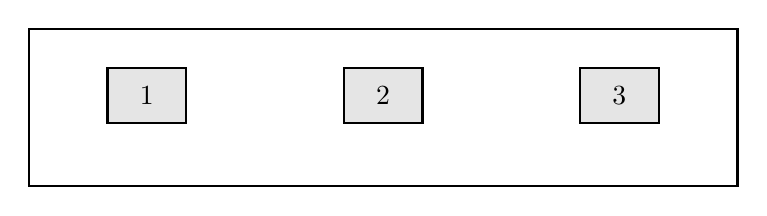
\begin{tikzpicture}
                \draw[thick] (0,0) rectangle (9,2);

                \foreach \x/\n in {1.0/1,4.0/2,7.0/3}{
                    \draw[fill=gray!20, thick]
                    (\x,0.8) rectangle ++(1,0.7);
                    \node at (\x+0.5,1.15) {\n};
                }
            \end{tikzpicture}
        \end{center}

        Cada elemento recibe espacio alrededor.

        \begin{alertblock}{Observe}
            El espacio de los extremos suele ser menor
            que el espacio existente entre elementos.
        \end{alertblock}
    \end{frame}

    % ---------------------------------------------------------
    \begin{frame}[fragile]{justify-content: space-evenly}
        \begin{csscodedark}
            .contenedor {
                display: flex;
                justify-content: space-evenly;
            }
        \end{csscodedark}

        \begin{center}
            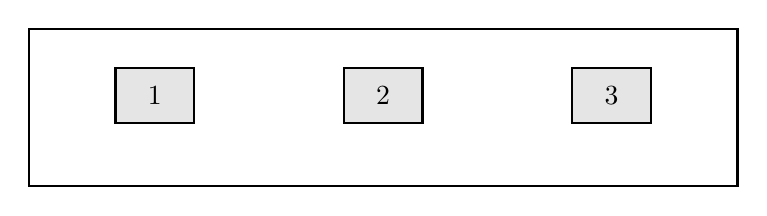
\begin{tikzpicture}
                \draw[thick] (0,0) rectangle (9,2);

                \foreach \x/\n in {1.1/1,4.0/2,6.9/3}{
                    \draw[fill=gray!20, thick]
                    (\x,0.8) rectangle ++(1,0.7);
                    \node at (\x+0.5,1.15) {\n};
                }
            \end{tikzpicture}
        \end{center}

        \begin{block}{Comportamiento}
            Los espacios entre elementos
            y en los extremos son uniformes.
        \end{block}
    \end{frame}

    % ---------------------------------------------------------
    \begin{frame}{Comparación de justify-content}
        \begin{center}
            \small
            \begin{tabular}{p{3.5cm}p{6.3cm}}
                \toprule
                \textbf{Valor} & \textbf{Resultado} \\
                \midrule

                \texttt{flex-start} &
                Elementos al inicio del eje. \\

                \texttt{center} &
                Elementos agrupados en el centro. \\

                \texttt{flex-end} &
                Elementos al final del eje. \\

                \texttt{space-between} &
                Espacio solamente entre elementos. \\

                \texttt{space-around} &
                Espacio alrededor de cada elemento. \\

                \texttt{space-evenly} &
                Espacios uniformes. \\

                \bottomrule
            \end{tabular}
        \end{center}
    \end{frame}


    % =========================================================
    % CAMBIO DEL EJE PRINCIPAL
    % =========================================================

    \begin{frame}[fragile]{¿Qué ocurre con column?}
        Cambiemos:

        \begin{csscodedark}
            .contenedor {
                display: flex;
                flex-direction: column;
            }
        \end{csscodedark}

        Ahora el eje principal es:

        \begin{center}
            \Large
            vertical
        \end{center}

        Por lo tanto:

        \begin{center}
            \texttt{justify-content}
        \end{center}

        controlará la distribución vertical.
    \end{frame}

    % ---------------------------------------------------------
    \begin{frame}{justify-content depende del eje}
        \begin{center}
            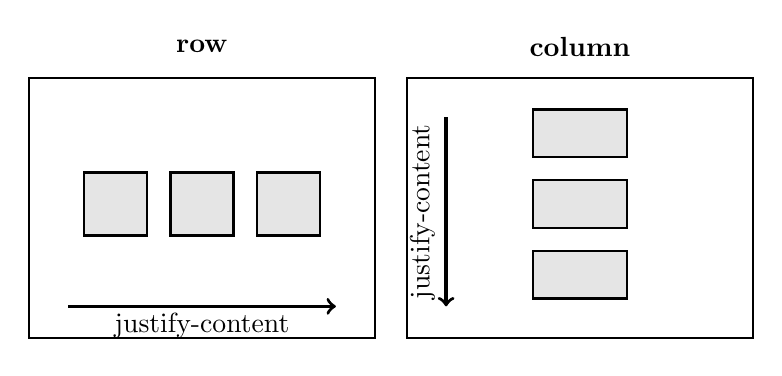
\begin{tikzpicture}

                % ROW
                \node at (2.2,4.4) {\textbf{row}};

                \draw[thick] (0,0.7) rectangle (4.4,4);

                \draw[->, very thick]
                (0.5,1.1) -- (3.9,1.1);

                \node at (2.2,0.85) {justify-content};

                \foreach \x in {0.7,1.8,2.9}{
                    \draw[fill=gray!20, thick]
                    (\x,2) rectangle ++(0.8,0.8);
                }

                % COLUMN
                \node at (7,4.4) {\textbf{column}};

                \draw[thick] (4.8,0.7) rectangle (9.2,4);

                \draw[->, very thick]
                (5.3,3.5) -- (5.3,1.1);

                \node[rotate=90] at (5,2.3) {justify-content};

                \foreach \y in {3.0,2.1,1.2}{
                    \draw[fill=gray!20, thick]
                    (6.4,\y) rectangle ++(1.2,0.6);
                }

            \end{tikzpicture}
        \end{center}

        \begin{alertblock}{No memorice ``horizontal''}
            Recuerde: \texttt{justify-content}
            trabaja sobre el \textbf{eje principal}.
        \end{alertblock}
    \end{frame}


    % =========================================================
    % ALIGN-ITEMS
    % =========================================================

    \section{align-items}

    \SectionSlide
    {align-items}
    {Alinear elementos sobre el eje transversal}

    % ---------------------------------------------------------
    \begin{frame}{¿Qué hace align-items?}
        La propiedad \texttt{align-items}
        controla la alineación de los elementos
        sobre el \textbf{eje transversal}.

        Si tenemos:

        \begin{center}
            \texttt{flex-direction: row;}
        \end{center}

        entonces:

        \begin{itemize}
            \item eje principal: horizontal;
            \item eje transversal: vertical.
        \end{itemize}

        \begin{block}{Sintaxis}
            \texttt{align-items: valor;}
        \end{block}
    \end{frame}

    % ---------------------------------------------------------
    \begin{frame}{Valores principales de align-items}
        Trabajaremos inicialmente con:

        \begin{itemize}
            \item \texttt{stretch}
            \item \texttt{flex-start}
            \item \texttt{center}
            \item \texttt{flex-end}
        \end{itemize}

        También existe:

        \begin{center}
            \texttt{baseline}
        \end{center}

        que veremos brevemente.
    \end{frame}

    % ---------------------------------------------------------
    \begin{frame}[fragile]{Necesitamos altura para observarlo}
        Para visualizar mejor \texttt{align-items},
        damos altura al contenedor:

        \begin{csscodedark}
            .contenedor {
                display: flex;
                height: 250px;
                border: 2px solid black;
            }
        \end{csscodedark}

        \begin{block}{¿Por qué?}
            Necesitamos espacio disponible
            sobre el eje transversal para observar
            cómo cambia la alineación.
        \end{block}
    \end{frame}

    % ---------------------------------------------------------
    \begin{frame}[fragile]{align-items: flex-start}
        \begin{csscodedark}
            .contenedor {
                display: flex;
                height: 250px;
                align-items: flex-start;
            }
        \end{csscodedark}

        \begin{center}
            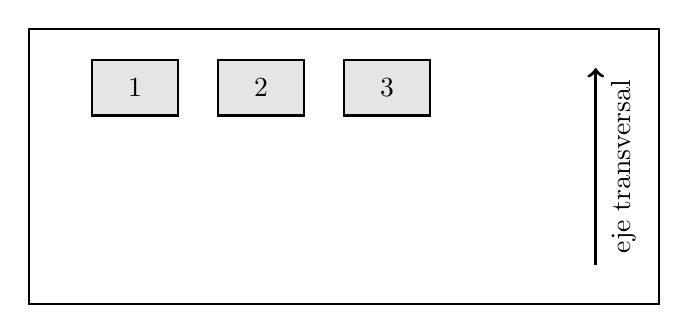
\begin{tikzpicture}
                \draw[thick] (0,0) rectangle (8,3.5);

                \foreach \x/\n in {0.8/1,2.4/2,4.0/3}{
                    \draw[fill=gray!20, thick]
                    (\x,2.4) rectangle ++(1.1,0.7);
                    \node at (\x+0.55,2.75) {\n};
                }

                \draw[->, very thick]
                (7.2,0.5) -- (7.2,3);
                \node[rotate=90] at (7.55,1.75) {eje transversal};
            \end{tikzpicture}
        \end{center}

        Los elementos se ubican al inicio
        del eje transversal.
    \end{frame}

    % ---------------------------------------------------------
    \begin{frame}[fragile]{align-items: center}
        Cambiamos solamente:

        \begin{csscodedark}
            .contenedor {
                display: flex;
                height: 250px;
                align-items: center;
            }
        \end{csscodedark}

        \begin{center}
            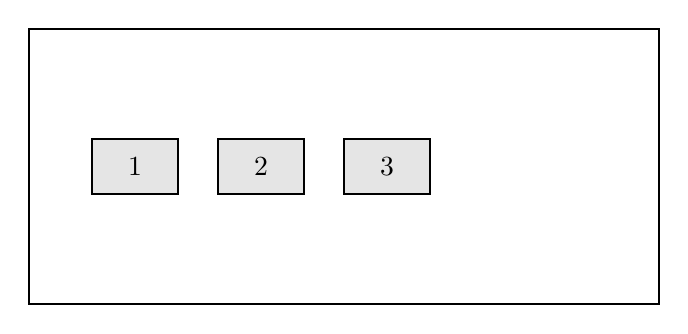
\begin{tikzpicture}
                \draw[thick] (0,0) rectangle (8,3.5);

                \foreach \x/\n in {0.8/1,2.4/2,4.0/3}{
                    \draw[fill=gray!20, thick]
                    (\x,1.4) rectangle ++(1.1,0.7);
                    \node at (\x+0.55,1.75) {\n};
                }
            \end{tikzpicture}
        \end{center}

        Los elementos se centran sobre
        el eje transversal.
    \end{frame}

    % ---------------------------------------------------------
    \begin{frame}[fragile]{align-items: flex-end}
        \begin{csscodedark}
            .contenedor {
                display: flex;
                height: 250px;
                align-items: flex-end;
            }
        \end{csscodedark}

        \begin{center}
            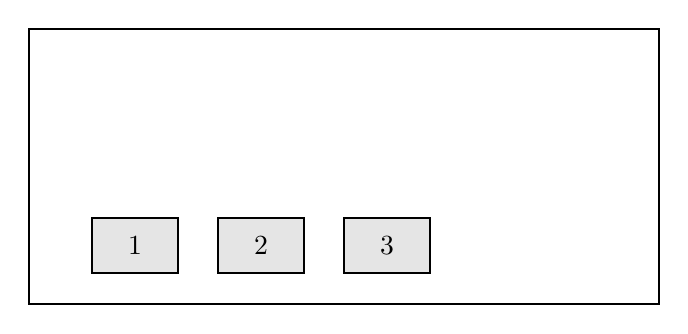
\begin{tikzpicture}
                \draw[thick] (0,0) rectangle (8,3.5);

                \foreach \x/\n in {0.8/1,2.4/2,4.0/3}{
                    \draw[fill=gray!20, thick]
                    (\x,0.4) rectangle ++(1.1,0.7);
                    \node at (\x+0.55,0.75) {\n};
                }
            \end{tikzpicture}
        \end{center}

        Los elementos se ubican al final
        del eje transversal.
    \end{frame}

    % ---------------------------------------------------------
    \begin{frame}[fragile]{align-items: stretch}
        \texttt{stretch} es el valor inicial.

        \begin{csscodedark}
            .contenedor {
                display: flex;
                height: 250px;
                align-items: stretch;
            }
        \end{csscodedark}

        Si los elementos no tienen una dimensión
        definida sobre el eje transversal,
        pueden estirarse para ocupar el espacio disponible.

        \begin{alertblock}{Importante}
            Si el elemento ya tiene una altura definida,
            el efecto puede ser diferente.
        \end{alertblock}
    \end{frame}

    % ---------------------------------------------------------
    \begin{frame}{Representación de stretch}
        \begin{center}
            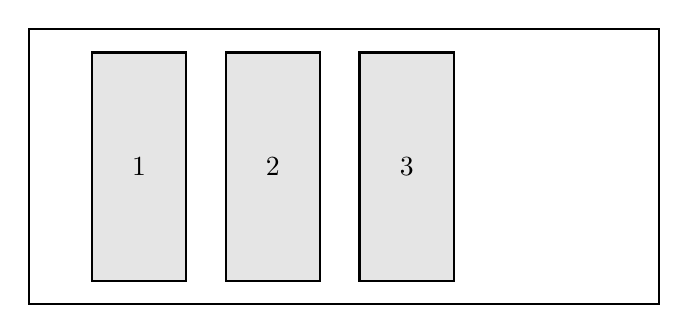
\begin{tikzpicture}
                \draw[thick] (0,0) rectangle (8,3.5);

                \foreach \x/\n in {0.8/1,2.5/2,4.2/3}{
                    \draw[fill=gray!20, thick]
                    (\x,0.3) rectangle ++(1.2,2.9);
                    \node at (\x+0.6,1.75) {\n};
                }
            \end{tikzpicture}
        \end{center}

        \begin{block}{Idea}
            \texttt{stretch} aprovecha el espacio
            disponible sobre el eje transversal.
        \end{block}
    \end{frame}

    % ---------------------------------------------------------
    \begin{frame}[fragile]{align-items: baseline}
        Otro valor disponible es:

        \begin{csscodedark}
            .contenedor {
                display: flex;
                align-items: baseline;
            }
        \end{csscodedark}

        Busca alinear los elementos teniendo en cuenta
        la línea base del contenido textual.

        \begin{block}{Uso}
            Puede resultar útil cuando los elementos
            contienen texto de diferentes tamaños.
        \end{block}
    \end{frame}


    % =========================================================
    % JUSTIFY VS ALIGN
    % =========================================================

    \section{Justify y Align}

    \SectionSlide
    {justify-content y align-items}
    {No confundir los dos ejes}

    % ---------------------------------------------------------
    \begin{frame}{La diferencia fundamental}
        \begin{center}
            \Large
            \texttt{justify-content}

            \vspace{0.2cm}

            $\downarrow$

            \textbf{eje principal}

            \vspace{0.7cm}

            \texttt{align-items}

            \vspace{0.2cm}

            $\downarrow$

            \textbf{eje transversal}
        \end{center}
    \end{frame}

    % ---------------------------------------------------------
    \begin{frame}{Mapa visual de los ejes}
        \begin{center}
            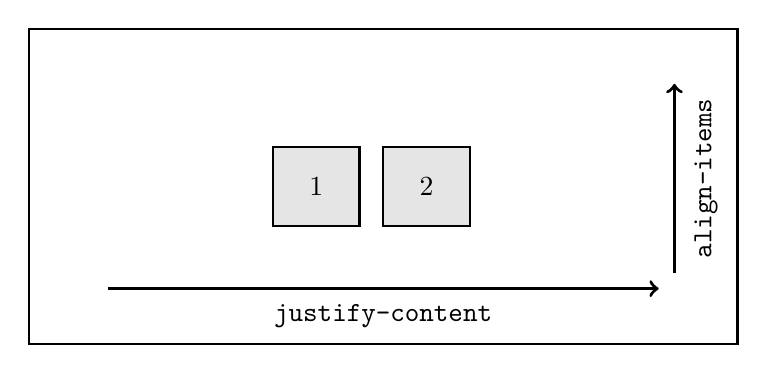
\begin{tikzpicture}
                \draw[thick] (0,0) rectangle (9,4);

                \draw[fill=gray!20, thick]
                (3.1,1.5) rectangle (4.2,2.5);
                \node at (3.65,2) {1};

                \draw[fill=gray!20, thick]
                (4.5,1.5) rectangle (5.6,2.5);
                \node at (5.05,2) {2};

                \draw[->, very thick]
                (1,0.7) -- (8,0.7);
                \node at (4.5,0.35)
                {\texttt{justify-content}};

                \draw[->, very thick]
                (8.2,0.9) -- (8.2,3.3);
                \node[rotate=90] at (8.6,2.1)
                {\texttt{align-items}};
            \end{tikzpicture}
        \end{center}

        Caso mostrado:

        \begin{center}
            \texttt{flex-direction: row;}
        \end{center}
    \end{frame}

    % ---------------------------------------------------------
    \begin{frame}[fragile]{Centrar horizontal y verticalmente}
        Ya podemos comprender este código:

        \begin{csscodedark}
            .contenedor {
                display: flex;
                justify-content: center;
                align-items: center;
            }
        \end{csscodedark}

        Con \texttt{flex-direction: row}:

        \begin{itemize}
            \item \texttt{justify-content: center}
            centra sobre el eje horizontal.
            \item \texttt{align-items: center}
            centra sobre el eje vertical.
        \end{itemize}
    \end{frame}

    % ---------------------------------------------------------
    \begin{frame}{Centrado en ambos ejes}
        \begin{center}
            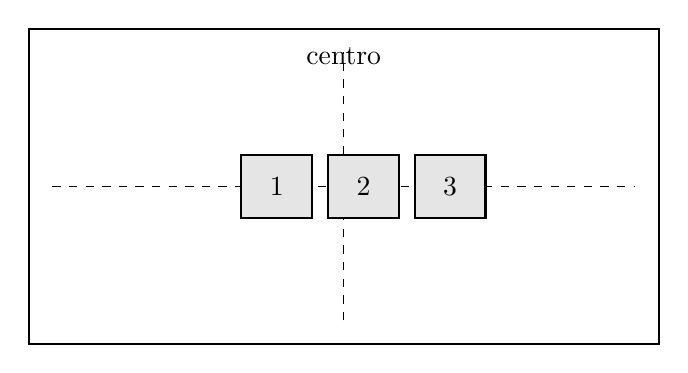
\begin{tikzpicture}
                \draw[thick] (0,0) rectangle (8,4);

                \draw[dashed] (4,0.3) -- (4,3.7);
                \draw[dashed] (0.3,2) -- (7.7,2);

                \foreach \x/\n in {2.7/1,3.8/2,4.9/3}{
                    \draw[fill=gray!20, thick]
                    (\x,1.6) rectangle ++(0.9,0.8);
                    \node at (\x+0.45,2) {\n};
                }

                \node at (4,3.65) {centro};
            \end{tikzpicture}
        \end{center}
    \end{frame}

    % ---------------------------------------------------------
    \begin{frame}[fragile]{¿Y si usamos column?}
        Ahora:

        \begin{csscodedark}
            .contenedor {
                display: flex;
                flex-direction: column;
                justify-content: center;
                align-items: center;
            }
        \end{csscodedark}

        \begin{block}{Cambio importante}
            El eje principal ahora es vertical.

            Por tanto, \texttt{justify-content}
            centra verticalmente.
        \end{block}
    \end{frame}

    % ---------------------------------------------------------
    \begin{frame}{La regla que debemos recordar}
        No memorice:

        \begin{center}
            \texttt{justify = horizontal}

            \texttt{align = vertical}
        \end{center}

        Eso solamente funciona cuando:

        \begin{center}
            \texttt{flex-direction: row}
        \end{center}

        Recuerde mejor:

        \begin{center}
            \Large
            justify $\rightarrow$ eje principal

            align $\rightarrow$ eje transversal
        \end{center}
    \end{frame}


    % =========================================================
    % GAP
    % =========================================================

    \section{gap}

    \SectionSlide
    {gap}
    {Separar elementos flex}

    % ---------------------------------------------------------
    \begin{frame}{¿Qué problema resuelve gap?}
        Cuando varios elementos están juntos,
        normalmente necesitamos separación entre ellos.

        Podríamos utilizar \texttt{margin},
        pero Flexbox proporciona una propiedad específica:

        \begin{center}
            \Large
            \texttt{gap}
        \end{center}

        \begin{block}{Función}
            \texttt{gap} define el espacio
            entre los elementos flex.
        \end{block}
    \end{frame}

    % ---------------------------------------------------------
    \begin{frame}[fragile]{Sintaxis de gap}
        Ejemplo:

        \begin{csscodedark}
            .contenedor {
                display: flex;
                gap: 20px;
            }
        \end{csscodedark}

        \begin{center}
            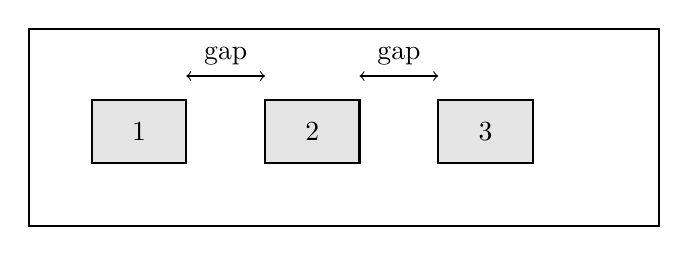
\begin{tikzpicture}
                \draw[thick] (0,0) rectangle (8,2.5);

                \draw[fill=gray!20, thick]
                (0.8,0.8) rectangle ++(1.2,0.8);
                \node at (1.4,1.2) {1};

                \draw[<->] (2,1.9) -- (3,1.9);
                \node at (2.5,2.15) {gap};

                \draw[fill=gray!20, thick]
                (3,0.8) rectangle ++(1.2,0.8);
                \node at (3.6,1.2) {2};

                \draw[<->] (4.2,1.9) -- (5.2,1.9);
                \node at (4.7,2.15) {gap};

                \draw[fill=gray!20, thick]
                (5.2,0.8) rectangle ++(1.2,0.8);
                \node at (5.8,1.2) {3};
            \end{tikzpicture}
        \end{center}
    \end{frame}

    % ---------------------------------------------------------
    \begin{frame}{Gap frente a margin}
        \begin{center}
            \small
            \begin{tabular}{p{3cm}p{3.6cm}p{3.6cm}}
                \toprule
                & \textbf{gap} & \textbf{margin} \\
                \midrule

                Función &
                Separar elementos &
                Espacio exterior \\

                Se aplica normalmente en &
                Contenedor &
                Elemento \\

                Afecta extremos automáticamente &
                No &
                Puede hacerlo \\

                Uso en Flexbox &
                Muy conveniente &
                También posible \\

                \bottomrule
            \end{tabular}
        \end{center}
    \end{frame}

    % ---------------------------------------------------------
    \begin{frame}[fragile]{Modificación progresiva}
        Antes:

        \begin{csscodedark}
            .contenedor {
                display: flex;
            }
        \end{csscodedark}

        Después:

        \begin{csscodedark}
            .contenedor {
                display: flex;
                gap: 20px;
            }
        \end{csscodedark}

        \begin{block}{Observe}
            No fue necesario modificar cada
            elemento \texttt{.caja}.
        \end{block}
    \end{frame}


    % =========================================================
    % FLEX-WRAP
    % =========================================================

    \section{flex-wrap}

    \SectionSlide
    {flex-wrap}
    {Permitir que los elementos cambien de línea}

    % ---------------------------------------------------------
    \begin{frame}{¿Qué ocurre cuando no hay espacio?}
        Por defecto, Flexbox intenta mantener
        todos los elementos dentro de una sola línea.

        Esto puede provocar que:

        \begin{itemize}
            \item Los elementos se reduzcan.
            \item El contenido quede muy comprimido.
            \item La distribución no sea conveniente.
        \end{itemize}

        \begin{block}{Solución}
            Podemos permitir varias líneas
            mediante \texttt{flex-wrap}.
        \end{block}
    \end{frame}

    % ---------------------------------------------------------
    \begin{frame}{Valores principales de flex-wrap}
        Los valores más importantes son:

        \begin{itemize}
            \item \texttt{nowrap}
            \item \texttt{wrap}
            \item \texttt{wrap-reverse}
        \end{itemize}

        \begin{block}{Valor predeterminado}
            \texttt{flex-wrap: nowrap;}
        \end{block}
    \end{frame}

    % ---------------------------------------------------------
    \begin{frame}[fragile]{flex-wrap: nowrap}
        Ejemplo:

        \begin{csscodedark}
            .contenedor {
                display: flex;
                flex-wrap: nowrap;
            }

            .caja {
                width: 200px;
            }
        \end{csscodedark}

        Flexbox intenta conservar los elementos
        en una única línea.

        \begin{alertblock}{Importante}
            Los elementos flex pueden reducirse
            si no existe espacio suficiente.
        \end{alertblock}
    \end{frame}

    % ---------------------------------------------------------
    \begin{frame}{Representación de nowrap}
        \begin{center}
            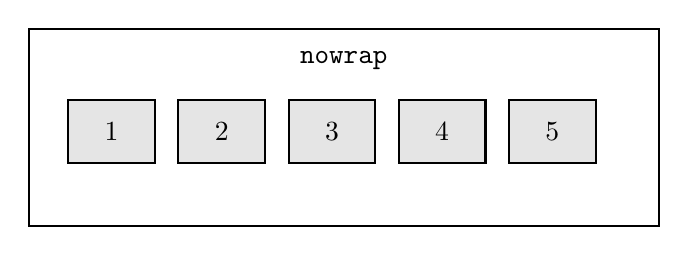
\begin{tikzpicture}
                \draw[thick] (0,0) rectangle (8,2.5);

                \foreach \x/\n in {0.5/1,1.9/2,3.3/3,4.7/4,6.1/5}{
                    \draw[fill=gray!20, thick]
                    (\x,0.8) rectangle ++(1.1,0.8);
                    \node at (\x+0.55,1.2) {\n};
                }

                \node at (4,2.1) {\texttt{nowrap}};
            \end{tikzpicture}
        \end{center}
    \end{frame}

    % ---------------------------------------------------------
    \begin{frame}[fragile]{flex-wrap: wrap}
        Modificamos:

        \begin{csscodedark}
            .contenedor {
                display: flex;
                flex-wrap: wrap;
            }

            .caja {
                width: 200px;
            }
        \end{csscodedark}

        \begin{block}{Resultado}
            Cuando los elementos dejan de caber,
            pueden continuar en una nueva línea.
        \end{block}
    \end{frame}

    % ---------------------------------------------------------
    \begin{frame}{Representación de wrap}
        \begin{center}
            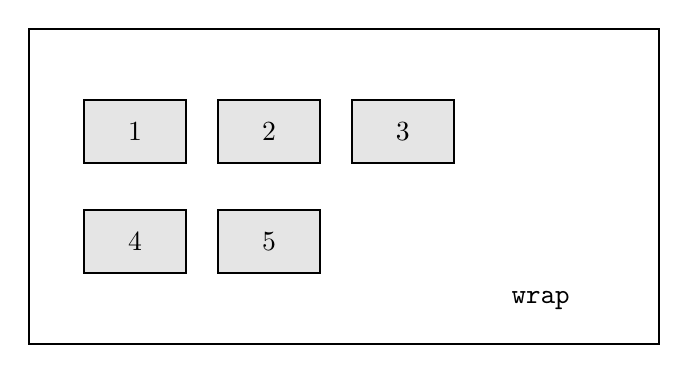
\begin{tikzpicture}
                \draw[thick] (0,0) rectangle (8,4);

                \foreach \x/\n in {0.7/1,2.4/2,4.1/3}{
                    \draw[fill=gray!20, thick]
                    (\x,2.3) rectangle ++(1.3,0.8);
                    \node at (\x+0.65,2.7) {\n};
                }

                \foreach \x/\n in {0.7/4,2.4/5}{
                    \draw[fill=gray!20, thick]
                    (\x,0.9) rectangle ++(1.3,0.8);
                    \node at (\x+0.65,1.3) {\n};
                }

                \node at (6.5,0.55) {\texttt{wrap}};
            \end{tikzpicture}
        \end{center}

        Los elementos continúan en otra línea
        cuando no existe espacio suficiente.
    \end{frame}

    % ---------------------------------------------------------
    \begin{frame}[fragile]{flex-wrap: wrap-reverse}
        También existe:

        \begin{csscodedark}
            .contenedor {
                display: flex;
                flex-wrap: wrap-reverse;
            }
        \end{csscodedark}

        Permite varias líneas,
        pero invierte la dirección
        en la que se generan esas líneas.

        \begin{block}{Uso inicial}
            Es menos frecuente que \texttt{wrap},
            pero forma parte de los valores disponibles.
        \end{block}
    \end{frame}


    % =========================================================
    % GAP + WRAP
    % =========================================================

    \begin{frame}[fragile]{Combinar gap y wrap}
        Ahora podemos combinar dos conceptos ya estudiados:

        \begin{csscodedark}
            .contenedor {
                display: flex;
                flex-wrap: wrap;
                gap: 20px;
            }
        \end{csscodedark}

        \begin{block}{Resultado}
            Los elementos pueden cambiar de línea
            y mantienen una separación uniforme.
        \end{block}
    \end{frame}

    % ---------------------------------------------------------
    \begin{frame}{Representación de gap + wrap}
        \begin{center}
            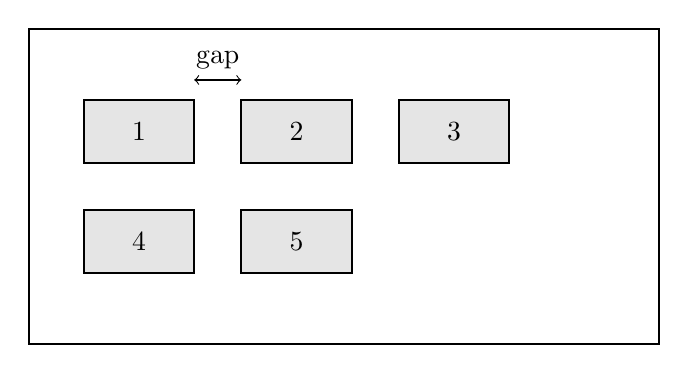
\begin{tikzpicture}
                \draw[thick] (0,0) rectangle (8,4);

                \draw[fill=gray!20, thick]
                (0.7,2.3) rectangle ++(1.4,0.8);
                \node at (1.4,2.7) {1};

                \draw[fill=gray!20, thick]
                (2.7,2.3) rectangle ++(1.4,0.8);
                \node at (3.4,2.7) {2};

                \draw[fill=gray!20, thick]
                (4.7,2.3) rectangle ++(1.4,0.8);
                \node at (5.4,2.7) {3};

                \draw[fill=gray!20, thick]
                (0.7,0.9) rectangle ++(1.4,0.8);
                \node at (1.4,1.3) {4};

                \draw[fill=gray!20, thick]
                (2.7,0.9) rectangle ++(1.4,0.8);
                \node at (3.4,1.3) {5};

                \draw[<->] (2.1,3.35) -- (2.7,3.35);
                \node at (2.4,3.6) {gap};
            \end{tikzpicture}
        \end{center}
    \end{frame}


    % =========================================================
    % EJEMPLO PROGRESIVO
    % =========================================================

    \section{Ejemplo progresivo}

    \SectionSlide
    {Ejemplo progresivo}
    {Construir un pequeño menú con Flexbox}

    % ---------------------------------------------------------
    \begin{frame}[fragile]{Paso 1: HTML}
        Utilicemos un menú pequeño:

        \begin{htmlcodedark}
            <nav class="menu">
            <a href="#">Inicio</a>
            <a href="#">Servicios</a>
            <a href="#">Contacto</a>
            </nav>
        \end{htmlcodedark}

        \begin{block}{Estructura}
            \texttt{nav} será el contenedor.

            Los enlaces serán sus elementos hijos.
        \end{block}
    \end{frame}

    % ---------------------------------------------------------
    \begin{frame}[fragile]{Paso 2: activar Flexbox}
        Primero:

        \begin{csscodedark}
            .menu {
                display: flex;
            }
        \end{csscodedark}

        Los enlaces pasan a ser
        elementos flex.
    \end{frame}

    % ---------------------------------------------------------
    \begin{frame}[fragile]{Paso 3: separar los enlaces}
        Agregamos:

        \begin{csscodedark}
            .menu {
                display: flex;
                gap: 20px;
            }
        \end{csscodedark}

        Ahora existe espacio uniforme
        entre los enlaces.
    \end{frame}

    % ---------------------------------------------------------
    \begin{frame}[fragile]{Paso 4: centrar el menú}
        Agregamos:

        \begin{csscodedark}
            .menu {
                display: flex;
                gap: 20px;
                justify-content: center;
            }
        \end{csscodedark}

        \begin{block}{Pregunta}
            ¿Sobre qué eje se está realizando
            el centrado?
        \end{block}
    \end{frame}

    % ---------------------------------------------------------
    \begin{frame}[fragile]{Paso 5: altura del menú}
        Ahora:

        \begin{csscodedark}
            .menu {
                display: flex;
                gap: 20px;
                justify-content: center;
                height: 80px;
            }
        \end{csscodedark}

        Todavía los elementos no están necesariamente
        centrados sobre el eje transversal.
    \end{frame}

    % ---------------------------------------------------------
    \begin{frame}[fragile]{Paso 6: centrar en ambos ejes}
        Finalmente:

        \begin{csscodedark}
            .menu {
                display: flex;
                gap: 20px;
                justify-content: center;
                align-items: center;
                height: 80px;
            }
        \end{csscodedark}

        \begin{block}{Resultado}
            Los enlaces quedan centrados
            sobre ambos ejes.
        \end{block}
    \end{frame}

    % ---------------------------------------------------------
    \begin{frame}{Análisis del menú}
        En:

        \begin{center}
            \texttt{flex-direction: row}
        \end{center}

        tenemos:

        \begin{description}
            \item[\texttt{display: flex}:]
            activa Flexbox.

            \item[\texttt{gap}:]
            separa los enlaces.

            \item[\texttt{justify-content}:]
            distribuye horizontalmente.

            \item[\texttt{align-items}:]
            alinea verticalmente.
        \end{description}
    \end{frame}


    % =========================================================
    % MINI PRÁCTICA
    % =========================================================

    \section{Aplicación del bloque}

    \SectionSlide
    {Aplicación}
    {Distribuir tarjetas sencillas}

    % ---------------------------------------------------------
    \begin{frame}[fragile]{HTML inicial}
        Utilice:

        \begin{htmlcodedark}
            <section class="tarjetas">

            <article class="tarjeta">
            <h2>Servicio 1</h2>
            </article>

            <article class="tarjeta">
            <h2>Servicio 2</h2>
            </article>

            <article class="tarjeta">
            <h2>Servicio 3</h2>
            </article>

            </section>
        \end{htmlcodedark}
    \end{frame}

    % ---------------------------------------------------------
    \begin{frame}[fragile]{Paso 1: hacer visibles las tarjetas}
        \begin{csscodedark}
            .tarjeta {
                width: 200px;
                padding: 20px;
                border: 1px solid gray;
            }
        \end{csscodedark}

        Observe primero el comportamiento
        antes de aplicar Flexbox.
    \end{frame}

    % ---------------------------------------------------------
    \begin{frame}[fragile]{Paso 2: activar Flexbox}
        \begin{csscodedark}
            .tarjetas {
                display: flex;
            }
        \end{csscodedark}

        \begin{block}{Observe}
            ¿Qué cambió respecto al flujo anterior?
        \end{block}
    \end{frame}

    % ---------------------------------------------------------
    \begin{frame}[fragile]{Paso 3: agregar separación}
        \begin{csscodedark}
            .tarjetas {
                display: flex;
                gap: 20px;
            }
        \end{csscodedark}
    \end{frame}

    % ---------------------------------------------------------
    \begin{frame}[fragile]{Paso 4: permitir varias líneas}
        \begin{csscodedark}
            .tarjetas {
                display: flex;
                gap: 20px;
                flex-wrap: wrap;
            }
        \end{csscodedark}

        Reduzca el ancho de la ventana
        y observe qué ocurre.
    \end{frame}

    % ---------------------------------------------------------
    \begin{frame}[fragile]{Paso 5: centrar las tarjetas}
        Agregue:

        \begin{csscodedark}
            .tarjetas {
                display: flex;
                gap: 20px;
                flex-wrap: wrap;
                justify-content: center;
            }
        \end{csscodedark}

        \begin{block}{Pregunta}
            ¿Por qué utilizamos
            \texttt{justify-content}
            y no \texttt{align-items}?
        \end{block}
    \end{frame}


    % =========================================================
    % ERRORES FRECUENTES DEL BLOQUE
    % =========================================================

    \section{Errores frecuentes}

    \SectionSlide
    {Errores frecuentes}
    {Comprender antes de combinar propiedades}

    % ---------------------------------------------------------
    \begin{frame}[fragile]{Aplicar justify-content al hijo}
        Incorrecto:

        \begin{csscodedark}
            .caja {
                justify-content: center;
            }
        \end{csscodedark}

        si \texttt{.caja} no es un contenedor flex.

        Correcto:

        \begin{csscodedark}
            .contenedor {
                display: flex;
                justify-content: center;
            }
        \end{csscodedark}

        \begin{alertblock}{Recuerde}
            Estas propiedades controlan
            la distribución de los hijos
            desde el contenedor.
        \end{alertblock}
    \end{frame}

    % ---------------------------------------------------------
    \begin{frame}{Confundir justify-content y align-items}
        Error frecuente:

        \begin{center}
            ``justify siempre es horizontal''
        \end{center}

        Esto es falso.

        La interpretación depende de:

        \begin{center}
            \Large
            \texttt{flex-direction}
        \end{center}

        \begin{block}{Regla correcta}
            justify $\rightarrow$ eje principal

            align $\rightarrow$ eje transversal
        \end{block}
    \end{frame}

    % ---------------------------------------------------------
    \begin{frame}[fragile]{Usar margin para cada separación}
        Esto funciona:

        \begin{csscodedark}
            .caja {
                margin-right: 20px;
            }
        \end{csscodedark}

        Pero cuando el objetivo es simplemente
        separar elementos flex, suele ser más claro:

        \begin{csscodedark}
            .contenedor {
                display: flex;
                gap: 20px;
            }
        \end{csscodedark}
    \end{frame}

    % ---------------------------------------------------------
    \begin{frame}[fragile]{Esperar wrap sin activarlo}
        Con:

        \begin{csscodedark}
            .contenedor {
                display: flex;
            }
        \end{csscodedark}

        el valor inicial es:

        \begin{center}
            \texttt{flex-wrap: nowrap;}
        \end{center}

        Si queremos varias líneas:

        \begin{csscodedark}
            .contenedor {
                display: flex;
                flex-wrap: wrap;
            }
        \end{csscodedark}
    \end{frame}

    % ---------------------------------------------------------
    \begin{frame}{Verificación del Bloque 2}
        El aprendiz debe poder explicar:

        \begin{itemize}
            \item Qué eje controla \texttt{justify-content}.
            \item Qué eje controla \texttt{align-items}.
            \item Por qué los ejes dependen de \texttt{flex-direction}.
            \item Diferencia entre \texttt{space-between},
            \texttt{space-around} y \texttt{space-evenly}.
            \item Qué función cumple \texttt{gap}.
            \item Qué diferencia existe entre \texttt{nowrap}
            y \texttt{wrap}.
            \item Por qué \texttt{display: flex}
            se aplica al contenedor.
        \end{itemize}
    \end{frame}

    % =========================================================
    % CLASE 6 - BLOQUE 3
    % ALIGN-CONTENT Y PROPIEDADES DE LOS ELEMENTOS FLEX
    % =========================================================

    % =========================================================
    % ALIGN-CONTENT
    % =========================================================

    \section{align-content}

    \SectionSlide
    {align-content}
    {Distribuir varias líneas dentro del contenedor}

    % ---------------------------------------------------------
    \begin{frame}{¿Qué hace align-content?}
        La propiedad \texttt{align-content}
        distribuye las \textbf{líneas flex}
        sobre el eje transversal.

        \begin{block}{Importante}
            Esta propiedad tiene sentido cuando:

            \begin{itemize}
                \item existe más de una línea;
                \item está activo \texttt{flex-wrap};
                \item existe espacio disponible en el contenedor.
            \end{itemize}
        \end{block}
    \end{frame}

    % ---------------------------------------------------------
    \begin{frame}[fragile]{HTML de referencia}
        Utilizaremos más elementos para provocar
        varias líneas:

        \begin{htmlcodedark}
        <div class="contenedor">
            <div class="caja">1</div>
            <div class="caja">2</div>
            <div class="caja">3</div>
            <div class="caja">4</div>
            <div class="caja">5</div>
            <div class="caja">6</div>
        </div>
        \end{htmlcodedark}
    \end{frame}

    % ---------------------------------------------------------
    \begin{frame}[fragile]{CSS inicial}
        \begin{csscodedark}
            .contenedor {
                display: flex;
                flex-wrap: wrap;
                height: 300px;
            }

            .caja {
                width: 180px;
            }
        \end{csscodedark}

        Ahora pueden existir varias líneas dentro
        de un contenedor con altura disponible.
    \end{frame}

    % ---------------------------------------------------------
    \begin{frame}{align-items frente a align-content}
        Estas propiedades no hacen lo mismo:

        \begin{description}
            \item[\texttt{align-items}:]
            alinea los elementos dentro de una línea flex.

            \item[\texttt{align-content}:]
            distribuye el conjunto de líneas flex
            cuando existen varias.
        \end{description}

        \begin{alertblock}{Regla práctica}
            Una línea $\rightarrow$ piense en \texttt{align-items}.

            Varias líneas $\rightarrow$ puede intervenir
            \texttt{align-content}.
        \end{alertblock}
    \end{frame}

    % ---------------------------------------------------------
    \begin{frame}{Representación conceptual}
        \begin{center}
            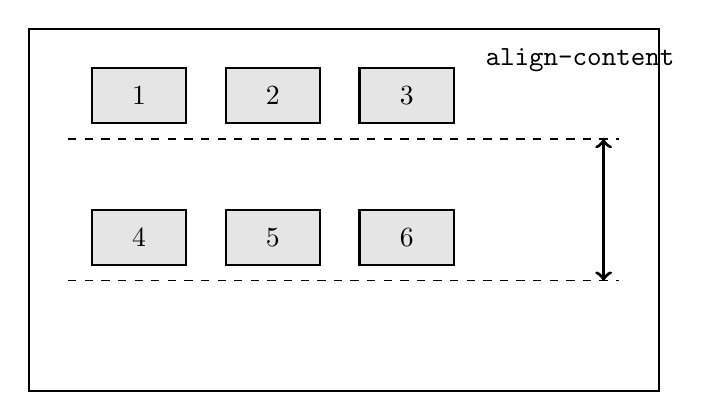
\begin{tikzpicture}
                \draw[thick] (0,0) rectangle (8,4.6);

                \node at (7,4.2) {\texttt{align-content}};

                % Primera línea
                \draw[dashed] (0.5,3.2) -- (7.5,3.2);

                \foreach \x/\n in {0.8/1,2.5/2,4.2/3}{
                    \draw[fill=gray!20, thick]
                    (\x,3.4) rectangle ++(1.2,0.7);
                    \node at (\x+0.6,3.75) {\n};
                }

                % Segunda línea
                \draw[dashed] (0.5,1.4) -- (7.5,1.4);

                \foreach \x/\n in {0.8/4,2.5/5,4.2/6}{
                    \draw[fill=gray!20, thick]
                    (\x,1.6) rectangle ++(1.2,0.7);
                    \node at (\x+0.6,1.95) {\n};
                }

                \draw[<->, very thick]
                (7.3,1.4) -- (7.3,3.2);
            \end{tikzpicture}
        \end{center}
    \end{frame}

    % ---------------------------------------------------------
    \begin{frame}{Valores principales de align-content}
        Podemos utilizar:

        \begin{itemize}
            \item \texttt{flex-start}
            \item \texttt{center}
            \item \texttt{flex-end}
            \item \texttt{space-between}
            \item \texttt{space-around}
            \item \texttt{space-evenly}
            \item \texttt{stretch}
        \end{itemize}
    \end{frame}

    % ---------------------------------------------------------
    \begin{frame}[fragile]{align-content: flex-start}
        \begin{csscodedark}
            .contenedor {
                display: flex;
                flex-wrap: wrap;
                height: 300px;
                align-content: flex-start;
            }
        \end{csscodedark}

        Las líneas se agrupan al inicio
        del eje transversal.
    \end{frame}

    % ---------------------------------------------------------
    \begin{frame}[fragile]{align-content: center}
        \begin{csscodedark}
            .contenedor {
                display: flex;
                flex-wrap: wrap;
                height: 300px;
                align-content: center;
            }
        \end{csscodedark}

        \begin{block}{Resultado}
            Las líneas flex se agrupan en el centro
            del eje transversal.
        \end{block}
    \end{frame}

    % ---------------------------------------------------------
    \begin{frame}[fragile]{align-content: space-between}
        \begin{csscodedark}
            .contenedor {
                display: flex;
                flex-wrap: wrap;
                height: 300px;
                align-content: space-between;
            }
        \end{csscodedark}

        La primera línea se ubica al inicio,
        la última al final y el espacio restante
        queda entre las líneas.
    \end{frame}

    % ---------------------------------------------------------
    \begin{frame}{align-items y align-content}
        \begin{center}
            \small
            \begin{tabular}{p{3.5cm}p{3.4cm}p{3.8cm}}
                \toprule
                & \textbf{align-items} & \textbf{align-content} \\
                \midrule

                Actúa sobre &
                Elementos &
                Líneas \\

                Requiere wrap &
                No &
                Normalmente sí \\

                Una sola línea &
                Sí tiene efecto &
                No suele tener efecto visible \\

                Eje &
                Transversal &
                Transversal \\

                \bottomrule
            \end{tabular}
        \end{center}
    \end{frame}


    % =========================================================
    % PROPIEDADES DE LOS ELEMENTOS FLEX
    % =========================================================

    \section{Elementos flex}

    \SectionSlide
    {Propiedades de los elementos flex}
    {Controlar el comportamiento de cada hijo}

    % ---------------------------------------------------------
    \begin{frame}{Propiedades del contenedor y de los hijos}
        Hasta ahora hemos aplicado propiedades
        principalmente al contenedor:

        \begin{itemize}
            \item \texttt{display}
            \item \texttt{flex-direction}
            \item \texttt{justify-content}
            \item \texttt{align-items}
            \item \texttt{gap}
            \item \texttt{flex-wrap}
            \item \texttt{align-content}
        \end{itemize}

        Ahora estudiaremos propiedades
        que se aplican a los \textbf{elementos flex}.
    \end{frame}

    % ---------------------------------------------------------
    \begin{frame}{Propiedades que estudiaremos}
        Sobre los elementos flex podemos utilizar:

        \begin{itemize}
            \item \texttt{flex-grow}
            \item \texttt{flex-shrink}
            \item \texttt{flex-basis}
            \item \texttt{flex}
            \item \texttt{order}
            \item \texttt{align-self}
        \end{itemize}

        \begin{block}{Diferencia}
            Estas propiedades se escriben normalmente
            en los elementos hijos, no en el contenedor.
        \end{block}
    \end{frame}


    % =========================================================
    % FLEX-GROW
    % =========================================================

    \section{flex-grow}

    \SectionSlide
    {flex-grow}
    {Distribuir el espacio disponible}

    % ---------------------------------------------------------
    \begin{frame}{¿Qué hace flex-grow?}
        \texttt{flex-grow} indica cuánto puede crecer
        un elemento flex cuando existe espacio disponible
        sobre el eje principal.

        \begin{block}{Valor inicial}
            \texttt{flex-grow: 0;}

            Los elementos no crecen automáticamente
            para ocupar el espacio restante.
        \end{block}
    \end{frame}

    % ---------------------------------------------------------
    \begin{frame}[fragile]{Ejemplo inicial}
        HTML:

        \begin{htmlcodedark}
        <div class="contenedor">
            <div class="caja">1</div>
            <div class="caja">2</div>
            <div class="caja">3</div>
        </div>
        \end{htmlcodedark}

        CSS:

        \begin{csscodedark}
            .contenedor {
                display: flex;
            }

            .caja {
                width: 100px;
            }
        \end{csscodedark}

        Si sobra espacio, este permanece libre.
    \end{frame}

    % ---------------------------------------------------------
    \begin{frame}[fragile]{Aplicar flex-grow}
        Modificamos los hijos:

        \begin{csscodedark}
            .caja {
                flex-grow: 1;
            }
        \end{csscodedark}

        \begin{block}{Resultado}
            Los tres elementos participan
            de manera equivalente en la distribución
            del espacio disponible.
        \end{block}
    \end{frame}

    % ---------------------------------------------------------
    \begin{frame}{Representación de flex-grow: 1}
        \begin{center}
            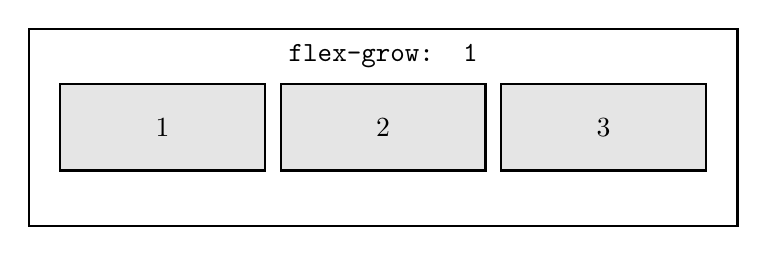
\begin{tikzpicture}
                \draw[thick] (0,0) rectangle (9,2.5);

                \draw[fill=gray!20, thick]
                (0.4,0.7) rectangle (3,1.8);
                \node at (1.7,1.25) {1};

                \draw[fill=gray!20, thick]
                (3.2,0.7) rectangle (5.8,1.8);
                \node at (4.5,1.25) {2};

                \draw[fill=gray!20, thick]
                (6,0.7) rectangle (8.6,1.8);
                \node at (7.3,1.25) {3};

                \node at (4.5,2.15) {\texttt{flex-grow: 1}};
            \end{tikzpicture}
        \end{center}
    \end{frame}

    % ---------------------------------------------------------
    \begin{frame}[fragile]{Un elemento puede crecer más}
        Podemos modificar solamente uno:

        \begin{csscodedark}
            .caja {
                flex-grow: 1;
            }

            .destacada {
                flex-grow: 2;
            }
        \end{csscodedark}

        HTML:

        \begin{htmlcodedark}
            <div class="caja">1</div>
            <div class="caja destacada">2</div>
            <div class="caja">3</div>
        \end{htmlcodedark}

        La caja 2 recibe una mayor proporción
        del espacio libre.
    \end{frame}

    % ---------------------------------------------------------
    \begin{frame}{Interpretación de flex-grow}
        Los valores representan proporciones
        del \textbf{espacio libre}, no necesariamente
        el ancho total de los elementos.

        Por ejemplo:

        \begin{center}
            \texttt{1 \qquad 2 \qquad 1}
        \end{center}

        significa que el espacio disponible
        se distribuye proporcionalmente
        en esas partes.

        \begin{alertblock}{Importante}
            \texttt{flex-grow: 2} no significa simplemente
            ``el elemento será el doble de ancho''.
        \end{alertblock}
    \end{frame}


    % =========================================================
    % FLEX-SHRINK
    % =========================================================

    \section{flex-shrink}

    \SectionSlide
    {flex-shrink}
    {Controlar la reducción de los elementos}

    % ---------------------------------------------------------
    \begin{frame}{¿Qué hace flex-shrink?}
        \texttt{flex-shrink} indica cuánto puede reducirse
        un elemento cuando no existe suficiente espacio.

        \begin{block}{Valor inicial}
            Normalmente:

            \texttt{flex-shrink: 1;}
        \end{block}

        Por eso los elementos flex pueden reducirse
        cuando el contenedor es pequeño.
    \end{frame}

    % ---------------------------------------------------------
    \begin{frame}[fragile]{Ejemplo}
        Supongamos:

        \begin{csscodedark}
            .contenedor {
                display: flex;
                width: 500px;
            }

            .caja {
                width: 250px;
            }
        \end{csscodedark}

        Tres cajas necesitarían inicialmente:

        \[
        250 + 250 + 250 = 750\text{px}
        \]

        pero el contenedor tiene solamente 500px.
    \end{frame}

    % ---------------------------------------------------------
    \begin{frame}[fragile]{Evitar que un elemento se reduzca}
        Podemos indicar:

        \begin{csscodedark}
            .importante {
                flex-shrink: 0;
            }
        \end{csscodedark}

        \begin{block}{Resultado}
            Ese elemento intenta conservar
            su tamaño base mientras otros elementos
            pueden absorber una mayor reducción.
        \end{block}
    \end{frame}

    % ---------------------------------------------------------
    \begin{frame}{grow frente a shrink}
        \begin{center}
            \begin{tabular}{p{3cm}p{3.5cm}p{3.5cm}}
                \toprule
                & \textbf{flex-grow} & \textbf{flex-shrink} \\
                \midrule

                Actúa cuando &
                Sobra espacio &
                Falta espacio \\

                Controla &
                Crecimiento &
                Reducción \\

                Valor inicial &
                \texttt{0} &
                \texttt{1} \\

                \bottomrule
            \end{tabular}
        \end{center}
    \end{frame}


    % =========================================================
    % FLEX-BASIS
    % =========================================================

    \section{flex-basis}

    \SectionSlide
    {flex-basis}
    {Definir el tamaño base del elemento flex}

    % ---------------------------------------------------------
    \begin{frame}{¿Qué hace flex-basis?}
        \texttt{flex-basis} define el tamaño inicial
        de un elemento sobre el eje principal
        antes de distribuir el espacio disponible.

        \begin{block}{Ejemplo}
            Con \texttt{flex-direction: row},
            el eje principal es horizontal.

            Por lo tanto, \texttt{flex-basis}
            influye inicialmente sobre el ancho.
        \end{block}
    \end{frame}

    % ---------------------------------------------------------
    \begin{frame}[fragile]{Ejemplo flex-basis}
        \begin{csscodedark}
            .caja {
                flex-basis: 200px;
            }
        \end{csscodedark}

        Esto establece una base inicial
        de 200px sobre el eje principal.
    \end{frame}

    % ---------------------------------------------------------
    \begin{frame}[fragile]{flex-basis con column}
        Si cambiamos:

        \begin{csscodedark}
            .contenedor {
                display: flex;
                flex-direction: column;
            }
        \end{csscodedark}

        entonces el eje principal pasa a ser vertical.

        \begin{block}{Consecuencia}
            \texttt{flex-basis} se relaciona ahora
            con el tamaño sobre ese eje vertical.
        \end{block}
    \end{frame}

    % ---------------------------------------------------------
    \begin{frame}{width frente a flex-basis}
        En una distribución flex horizontal:

        \begin{itemize}
            \item \texttt{width} define un ancho.
            \item \texttt{flex-basis} define la base
            utilizada por el algoritmo de Flexbox.
        \end{itemize}

        \begin{block}{Para aprender Flexbox}
            Cuando queremos controlar el tamaño base
            de un elemento flex, suele ser útil
            trabajar directamente con \texttt{flex-basis}.
        \end{block}
    \end{frame}


    % =========================================================
    % FLEX
    % =========================================================

    \section{Propiedad flex}

    \SectionSlide
    {Propiedad flex}
    {Forma abreviada de grow, shrink y basis}

    % ---------------------------------------------------------
    \begin{frame}{¿Qué es la propiedad flex?}
        \texttt{flex} permite escribir en una sola declaración:

        \begin{itemize}
            \item \texttt{flex-grow}
            \item \texttt{flex-shrink}
            \item \texttt{flex-basis}
        \end{itemize}

        Su estructura general es:

        \begin{center}
            \Large
            \texttt{flex: grow shrink basis;}
        \end{center}
    \end{frame}

    % ---------------------------------------------------------
    \begin{frame}[fragile]{Ejemplo completo}
        En lugar de:

        \begin{csscodedark}
            .caja {
                flex-grow: 1;
                flex-shrink: 1;
                flex-basis: 200px;
            }
        \end{csscodedark}

        podemos escribir:

        \begin{csscodedark}
            .caja {
                flex: 1 1 200px;
            }
        \end{csscodedark}
    \end{frame}

    % ---------------------------------------------------------
    \begin{frame}{Lectura de flex}
        En:

        \begin{center}
            \Large
            \texttt{flex: 1 1 200px;}
        \end{center}

        tenemos:

        \begin{description}
            \item[\texttt{1}:]
            flex-grow.

            \item[\texttt{1}:]
            flex-shrink.

            \item[\texttt{200px}:]
            flex-basis.
        \end{description}
    \end{frame}

    % ---------------------------------------------------------
    \begin{frame}[fragile]{Una forma muy utilizada}
        Es frecuente encontrar:

        \begin{csscodedark}
            .caja {
                flex: 1;
            }
        \end{csscodedark}

        Esta forma permite crear elementos
        que participan de manera flexible
        en el espacio disponible.

        \begin{alertblock}{Por ahora}
            Utilizaremos \texttt{flex: 1}
            principalmente para crear elementos
            que reparten el espacio disponible.
        \end{alertblock}
    \end{frame}


    % =========================================================
    % ORDER
    % =========================================================

    \section{order}

    \SectionSlide
    {order}
    {Modificar el orden visual}

    % ---------------------------------------------------------
    \begin{frame}{¿Qué hace order?}
        La propiedad \texttt{order} permite modificar
        el orden visual de un elemento flex.

        Por defecto:

        \begin{center}
            \texttt{order: 0;}
        \end{center}

        Los elementos con valores menores
        aparecen antes que aquellos
        con valores mayores.
    \end{frame}

    % ---------------------------------------------------------
    \begin{frame}[fragile]{Ejemplo}
        HTML:

        \begin{htmlcodedark}
            <div class="caja uno">1</div>
            <div class="caja dos">2</div>
            <div class="caja tres">3</div>
        \end{htmlcodedark}

        CSS:

        \begin{csscodedark}
            .tres {
                order: -1;
            }
        \end{csscodedark}

        La caja 3 puede aparecer visualmente
        antes que las demás.
    \end{frame}

    % ---------------------------------------------------------
    \begin{frame}{Orden HTML frente a orden visual}
        \begin{center}
            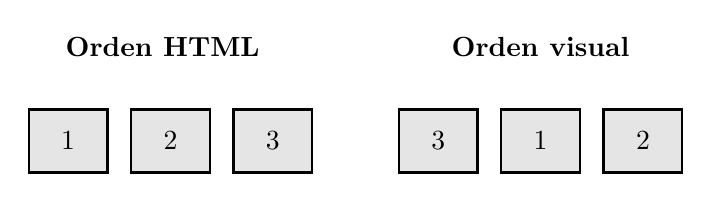
\begin{tikzpicture}

                \node at (2.2,3.6) {\textbf{Orden HTML}};

                \draw[fill=gray!20, thick]
                (0.5,2) rectangle (1.5,2.8);
                \node at (1,2.4) {1};

                \draw[fill=gray!20, thick]
                (1.8,2) rectangle (2.8,2.8);
                \node at (2.3,2.4) {2};

                \draw[fill=gray!20, thick]
                (3.1,2) rectangle (4.1,2.8);
                \node at (3.6,2.4) {3};

                \node at (7,3.6) {\textbf{Orden visual}};

                \draw[fill=gray!20, thick]
                (5.2,2) rectangle (6.2,2.8);
                \node at (5.7,2.4) {3};

                \draw[fill=gray!20, thick]
                (6.5,2) rectangle (7.5,2.8);
                \node at (7,2.4) {1};

                \draw[fill=gray!20, thick]
                (7.8,2) rectangle (8.8,2.8);
                \node at (8.3,2.4) {2};

            \end{tikzpicture}
        \end{center}

        \begin{alertblock}{Precaución}
            Cambiar el orden visual no modifica
            el orden real del documento HTML.
        \end{alertblock}
    \end{frame}

    % ---------------------------------------------------------
    \begin{frame}{Uso responsable de order}
        \texttt{order} puede ser útil para ajustes visuales,
        pero no debería utilizarse para corregir
        una estructura HTML mal organizada.

        \begin{block}{Buena práctica}
            El HTML debería conservar un orden lógico
            y comprensible incluso sin CSS.
        \end{block}
    \end{frame}


    % =========================================================
    % ALIGN-SELF
    % =========================================================

    \section{align-self}

    \SectionSlide
    {align-self}
    {Alinear un elemento de forma individual}

    % ---------------------------------------------------------
    \begin{frame}{¿Qué hace align-self?}
        \texttt{align-self} permite cambiar
        la alineación de un único elemento
        sobre el eje transversal.

        Puede sobrescribir para ese elemento
        el comportamiento definido mediante:

        \begin{center}
            \texttt{align-items}
        \end{center}
    \end{frame}

    % ---------------------------------------------------------
    \begin{frame}[fragile]{Ejemplo}
        Contenedor:

        \begin{csscodedark}
            .contenedor {
                display: flex;
                height: 250px;
                align-items: flex-start;
            }
        \end{csscodedark}

        Un elemento:

        \begin{csscodedark}
            .destacada {
                align-self: flex-end;
            }
        \end{csscodedark}
    \end{frame}

    % ---------------------------------------------------------
    \begin{frame}{Representación de align-self}
        \begin{center}
            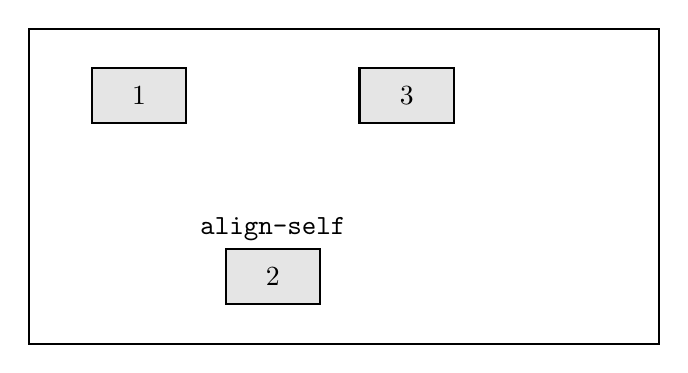
\begin{tikzpicture}
                \draw[thick] (0,0) rectangle (8,4);

                \draw[fill=gray!20, thick]
                (0.8,2.8) rectangle ++(1.2,0.7);
                \node at (1.4,3.15) {1};

                \draw[fill=gray!20, thick]
                (2.5,0.5) rectangle ++(1.2,0.7);
                \node at (3.1,0.85) {2};

                \draw[fill=gray!20, thick]
                (4.2,2.8) rectangle ++(1.2,0.7);
                \node at (4.8,3.15) {3};

                \node at (3.1,1.45) {\texttt{align-self}};
            \end{tikzpicture}
        \end{center}

        Solo la caja 2 cambia su alineación.
    \end{frame}


    % =========================================================
    % RESUMEN CONTENEDOR VS ELEMENTOS
    % =========================================================

    \section{Resumen de propiedades}

    \SectionSlide
    {Contenedor y elementos flex}
    {Identificar dónde se escribe cada propiedad}

    % ---------------------------------------------------------
    \begin{frame}{Propiedades del contenedor}
        Normalmente se escriben en el padre:

        \begin{itemize}
            \item \texttt{display: flex}
            \item \texttt{flex-direction}
            \item \texttt{justify-content}
            \item \texttt{align-items}
            \item \texttt{gap}
            \item \texttt{flex-wrap}
            \item \texttt{align-content}
        \end{itemize}
    \end{frame}

    % ---------------------------------------------------------
    \begin{frame}{Propiedades de los elementos}
        Normalmente se escriben en los hijos:

        \begin{itemize}
            \item \texttt{flex-grow}
            \item \texttt{flex-shrink}
            \item \texttt{flex-basis}
            \item \texttt{flex}
            \item \texttt{order}
            \item \texttt{align-self}
        \end{itemize}
    \end{frame}

    % ---------------------------------------------------------
    \begin{frame}{Mapa conceptual de Flexbox}
        \begin{center}
            \begin{tikzpicture}[
                caja/.style={
                    rectangle,
                    rounded corners,
                    draw,
                    thick,
                    align=center,
                    minimum width=3cm,
                    minimum height=0.8cm
                },
                flecha/.style={->, thick, >=Latex}
                ]

                \node[caja] (flex) {\textbf{Flexbox}};

                \node[caja, below left=1.6cm and 2cm of flex]
                (contenedor) {Contenedor flex};

                \node[caja, below right=1.6cm and 2cm of flex]
                (hijos) {Elementos flex};

                \draw[flecha] (flex) -- (contenedor);
                \draw[flecha] (flex) -- (hijos);

                \node[below=0.5cm of contenedor, align=center]
                {
                    direction\\
                    justify-content\\
                    align-items\\
                    wrap\\
                    gap
                };

                \node[below=0.5cm of hijos, align=center]
                {
                    grow\\
                    shrink\\
                    basis\\
                    order\\
                    align-self
                };

            \end{tikzpicture}
        \end{center}
    \end{frame}


    % =========================================================
    % PRÁCTICA GUIADA COMPLETA
    % =========================================================

    \section{Práctica guiada}

    \SectionSlide
    {Práctica guiada}
    {Sección de servicios}

    % ---------------------------------------------------------
    \begin{frame}{Contexto}
        Una empresa necesita presentar tres servicios
        mediante tarjetas.

        Construiremos una sección que:

        \begin{itemize}
            \item Organice tarjetas horizontalmente.
            \item Mantenga separación uniforme.
            \item Permita varias líneas.
            \item Distribuya el espacio disponible.
            \item Mantenga los botones alineados.
        \end{itemize}
    \end{frame}

    % ---------------------------------------------------------
    \begin{frame}[fragile]{Estructura del proyecto}
        Cree:

        \begin{bashcodedark}
            servicios-flex/
            ├── index.html
            └── css/
            └── styles.css
        \end{bashcodedark}
    \end{frame}

    % ---------------------------------------------------------
    \begin{frame}[fragile]{Paso 1: HTML}
        \begin{htmlcodedark}
    <section class="servicios">
        <article class="tarjeta">
            <h2>Diseño Web</h2>
            <p>Diseño de interfaces modernas.</p>
            <button>Consultar</button>
        </article>
        <article class="tarjeta">
            <h2>Soporte</h2>
            <p>Asistencia para plataformas digitales.</p>
            <button>Consultar</button>
        </article>
        <article class="tarjeta">
            <h2>Desarrollo</h2>
            <p>Construcción de aplicaciones web.</p>
            <button>Consultar</button>
        </article>
    </section>
        \end{htmlcodedark}
    \end{frame}

    % ---------------------------------------------------------
    \begin{frame}[fragile]{Paso 2: activar Flexbox}
        \begin{csscodedark}
            .servicios {
                display: flex;
            }
        \end{csscodedark}

        Observe el cambio en la distribución.
    \end{frame}

    % ---------------------------------------------------------
    \begin{frame}[fragile]{Paso 3: separación y wrap}
        Agregue:

        \begin{csscodedark}
            .servicios {
                display: flex;
                gap: 20px;
                flex-wrap: wrap;
            }
        \end{csscodedark}
    \end{frame}

    % ---------------------------------------------------------
    \begin{frame}[fragile]{Paso 4: tamaño base}
        Ahora aplicamos:

        \begin{csscodedark}
            .tarjeta {
                flex-basis: 250px;
                padding: 20px;
                border: 1px solid gray;
            }
        \end{csscodedark}

        \begin{block}{Observe}
            Cada tarjeta parte de una base
            aproximada de 250px.
        \end{block}
    \end{frame}

    % ---------------------------------------------------------
    \begin{frame}[fragile]{Paso 5: permitir crecimiento}
        Modifique:

        \begin{csscodedark}
            .tarjeta {
                flex-grow: 1;
                flex-basis: 250px;
            }
        \end{csscodedark}

        Ahora las tarjetas pueden utilizar
        el espacio disponible.
    \end{frame}

    % ---------------------------------------------------------
    \begin{frame}[fragile]{Paso 6: forma abreviada}
        Podemos reemplazar:

        \begin{csscodedark}
            .tarjeta {
                flex-grow: 1;
                flex-shrink: 1;
                flex-basis: 250px;
            }
        \end{csscodedark}

        por:

        \begin{csscodedark}
            .tarjeta {
                flex: 1 1 250px;
            }
        \end{csscodedark}
    \end{frame}

    % ---------------------------------------------------------
    \begin{frame}[fragile]{Paso 7: Flexbox dentro de la tarjeta}
        Una caja también puede convertirse
        en contenedor flex:

        \begin{csscodedark}
            .tarjeta {
                display: flex;
                flex-direction: column;
            }
        \end{csscodedark}

        \begin{block}{Importante}
            Un elemento puede ser simultáneamente:

            elemento flex de su padre

            y contenedor flex de sus propios hijos.
        \end{block}
    \end{frame}

    % ---------------------------------------------------------
    \begin{frame}[fragile]{Paso 8: enviar el botón al final}
        Aplicamos:

        \begin{csscodedark}
            .tarjeta button {
                margin-top: auto;
            }
        \end{csscodedark}

        \begin{block}{Resultado}
            El margen automático utiliza el espacio disponible
            y ayuda a mantener los botones hacia la parte inferior
            de las tarjetas.
        \end{block}
    \end{frame}

    % ---------------------------------------------------------
    \begin{frame}{Resultado conceptual}
        \begin{center}
            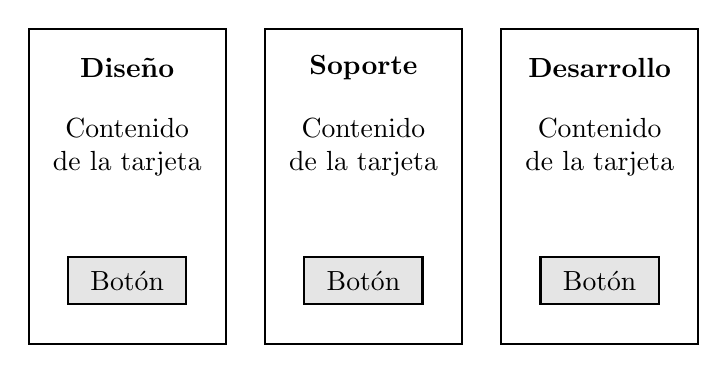
\begin{tikzpicture}

                \foreach \x/\titulo in {
                    0.2/Diseño,
                    3.2/Soporte,
                    6.2/Desarrollo
                }{
                    \draw[thick] (\x,0) rectangle ++(2.5,4);
                    \node at (\x+1.25,3.5) {\textbf{\titulo}};
                    \node[align=center] at (\x+1.25,2.5)
                    {Contenido\\de la tarjeta};

                    \draw[fill=gray!20, thick]
                    (\x+0.5,0.5) rectangle ++(1.5,0.6);

                    \node at (\x+1.25,0.8) {Botón};
                }

            \end{tikzpicture}
        \end{center}

        Los botones permanecen visualmente
        alineados en la parte inferior.
    \end{frame}

    % ---------------------------------------------------------
    \begin{frame}[fragile]{CSS principal de la práctica}
        \begin{csscodedark}
            .servicios {
                display: flex;
                flex-wrap: wrap;
                gap: 20px;
            }
            .tarjeta {
                flex: 1 1 250px;
                display: flex;
                flex-direction: column;
                padding: 20px;
                border: 1px solid gray;
            }
            .tarjeta button {
                margin-top: auto;
            }
        \end{csscodedark}
    \end{frame}


    % =========================================================
    % EJERCICIO AUTÓNOMO
    % =========================================================

    \section{Ejercicio autónomo}

    \SectionSlide
    {Ejercicio autónomo}
    {Catálogo de cursos}

    % ---------------------------------------------------------
    \begin{frame}{Situación propuesta}
        Construya una página para presentar
        un pequeño catálogo de cursos.

        Debe incluir al menos cuatro cursos,
        por ejemplo:

        \begin{itemize}
            \item Programación.
            \item Diseño.
            \item Bases de datos.
            \item Redes.
        \end{itemize}

        Cada curso debe mostrarse dentro
        de una tarjeta.
    \end{frame}

    % ---------------------------------------------------------
    \begin{frame}{Contenido de cada tarjeta}
        Cada tarjeta debe incluir:

        \begin{itemize}
            \item Nombre del curso.
            \item Descripción breve.
            \item Duración.
            \item Modalidad.
            \item Botón de información.
        \end{itemize}
    \end{frame}

    % ---------------------------------------------------------
    \begin{frame}{Requisitos Flexbox}
        Utilice como mínimo:

        \begin{itemize}
            \item \texttt{display: flex}.
            \item \texttt{flex-direction}.
            \item \texttt{justify-content}.
            \item \texttt{align-items}.
            \item \texttt{gap}.
            \item \texttt{flex-wrap}.
            \item \texttt{flex-basis} o \texttt{flex}.
        \end{itemize}
    \end{frame}

    % ---------------------------------------------------------
    \begin{frame}{Requisito adicional}
        Dentro de cada tarjeta:

        \begin{itemize}
            \item Utilice Flexbox en dirección vertical.
            \item Mantenga el botón hacia la parte inferior.
        \end{itemize}

        \begin{block}{Objetivo}
            Comprender que Flexbox puede utilizarse
            tanto para distribuir tarjetas como para organizar
            el contenido interno de cada tarjeta.
        \end{block}
    \end{frame}

    % ---------------------------------------------------------
    \begin{frame}[fragile]{Estructura de entrega}
        Organice el proyecto:

        \begin{bashcodedark}
            catalogo-cursos-nombre-apellido/
            ├── index.html
            └── css/
            └── styles.css
        \end{bashcodedark}
    \end{frame}

    % ---------------------------------------------------------
    \begin{frame}{Lista de verificación}
        Antes de entregar:

        \begin{itemize}
            \item El archivo CSS está correctamente conectado.
            \item Existe un contenedor flex principal.
            \item Las tarjetas pueden cambiar de línea.
            \item Existe separación mediante \texttt{gap}.
            \item Los elementos se distribuyen correctamente.
            \item Se utiliza correctamente el eje principal.
            \item Se utiliza correctamente el eje transversal.
            \item Las tarjetas tienen un tamaño base definido.
            \item El código HTML conserva un orden lógico.
            \item El aprendiz puede explicar cada propiedad utilizada.
        \end{itemize}
    \end{frame}


    % =========================================================
    % ERRORES FRECUENTES
    % =========================================================

    \section{Errores frecuentes}

    \SectionSlide
    {Errores frecuentes}
    {Problemas comunes con Flexbox}

    % ---------------------------------------------------------
    \begin{frame}[fragile]{Aplicar propiedades en el lugar incorrecto}
        Incorrecto:

        \begin{csscodedark}
            .caja {
                justify-content: center;
            }
        \end{csscodedark}

        si \texttt{.caja} solamente es un elemento flex.

        Para distribuir las cajas:

        \begin{csscodedark}
            .contenedor {
                display: flex;
                justify-content: center;
            }
        \end{csscodedark}
    \end{frame}

    % ---------------------------------------------------------
    \begin{frame}{Confundir contenedor e hijo}
        Recuerde:

        \begin{center}
            \Large
            Padre
            $\rightarrow$
            organiza

            \vspace{0.4cm}

            Hijo
            $\rightarrow$
            se adapta
        \end{center}

        Algunas propiedades pertenecen al contenedor
        y otras al elemento flex.
    \end{frame}

    % ---------------------------------------------------------
    \begin{frame}{Memorizar horizontal y vertical}
        Otro error es asumir:

        \begin{center}
            justify = horizontal

            align = vertical
        \end{center}

        La interpretación correcta es:

        \begin{center}
            justify $\rightarrow$ eje principal

            align $\rightarrow$ eje transversal
        \end{center}

        y ambos dependen de:

        \begin{center}
            \texttt{flex-direction}
        \end{center}
    \end{frame}

    % ---------------------------------------------------------
    \begin{frame}[fragile]{Esperar align-content con una sola línea}
        Si tenemos:

        \begin{csscodedark}
            .contenedor {
                display: flex;
                align-content: center;
            }
        \end{csscodedark}

        pero existe solamente una línea,
        probablemente no veremos el resultado esperado.

        \begin{block}{Recuerde}
            \texttt{align-content} trabaja
            con múltiples líneas flex.
        \end{block}
    \end{frame}

    % ---------------------------------------------------------
    \begin{frame}{Usar order para corregir HTML}
        Aunque CSS permite modificar
        el orden visual:

        \begin{center}
            \texttt{order}
        \end{center}

        el HTML debe seguir conservando
        una secuencia lógica.

        \begin{alertblock}{Buena práctica}
            No dependa de \texttt{order}
            para reparar una estructura HTML incorrecta.
        \end{alertblock}
    \end{frame}


    % =========================================================
    % CIERRE
    % =========================================================

    \section{Cierre}

    \SectionSlide
    {Cierre}
    {Resumen de Flexbox}

    % ---------------------------------------------------------
    \begin{frame}{¿Qué aprendimos?}
        Flexbox permite:

        \begin{itemize}
            \item Organizar elementos dentro de un contenedor.
            \item Cambiar la dirección del eje principal.
            \item Distribuir elementos sobre el eje principal.
            \item Alinear elementos sobre el eje transversal.
            \item Crear separaciones mediante \texttt{gap}.
            \item Permitir múltiples líneas mediante \texttt{flex-wrap}.
            \item Distribuir líneas mediante \texttt{align-content}.
            \item Controlar crecimiento y reducción.
            \item Definir tamaños base flexibles.
            \item Modificar individualmente ciertos elementos.
        \end{itemize}
    \end{frame}

    % ---------------------------------------------------------
    \begin{frame}{Mapa final de Flexbox}
        \begin{center}
            \resizebox{0.9\textwidth}{!}{%
                \begin{tikzpicture}[
                    caja/.style={
                        rectangle,
                        rounded corners,
                        draw,
                        thick,
                        align=center,
                        minimum width=3.3cm,
                        minimum height=0.8cm
                    },
                    flecha/.style={->, thick, >=Latex}
                    ]

                    \node[caja] (flex) {\textbf{Flexbox}};

                    \node[caja, below left=1.4cm and 2cm of flex]
                    (padre) {Contenedor};

                    \node[caja, below right=1.4cm and 2cm of flex]
                    (hijo) {Elementos};

                    \node[caja, below=1.4cm of padre]
                    (ejes) {Ejes y distribución};

                    \node[caja, below=1.4cm of hijo]
                    (tamano) {Tamaño y comportamiento};

                    \draw[flecha] (flex) -- (padre);
                    \draw[flecha] (flex) -- (hijo);
                    \draw[flecha] (padre) -- (ejes);
                    \draw[flecha] (hijo) -- (tamano);

                    \node[below=0.4cm of ejes, align=center]
                    {
                        direction\\
                        justify\\
                        align\\
                        wrap\\
                        gap
                    };

                    \node[below=0.4cm of tamano, align=center]
                    {
                        grow\\
                        shrink\\
                        basis\\
                        order\\
                        align-self
                    };

                \end{tikzpicture}
            }
        \end{center}
    \end{frame}

    % ---------------------------------------------------------
    \begin{frame}{Propiedades esenciales}
        \begin{center}
            \small
            \begin{tabular}{p{3.8cm}p{6cm}}
                \toprule
                \textbf{Propiedad} & \textbf{Función principal} \\
                \midrule

                \texttt{display: flex} &
                Activa Flexbox. \\

                \texttt{flex-direction} &
                Define el eje principal. \\

                \texttt{justify-content} &
                Distribuye sobre el eje principal. \\

                \texttt{align-items} &
                Alinea sobre el eje transversal. \\

                \texttt{gap} &
                Separa los elementos. \\

                \texttt{flex-wrap} &
                Permite varias líneas. \\

                \texttt{align-content} &
                Distribuye las líneas. \\

                \texttt{flex} &
                Controla crecimiento, reducción y base. \\

                \bottomrule
            \end{tabular}
        \end{center}
    \end{frame}

    % ---------------------------------------------------------
    \begin{frame}{¿Qué sigue?}
        Flexbox resulta especialmente útil
        cuando queremos organizar elementos
        principalmente en una dimensión.

        Sin embargo, algunas interfaces necesitan
        controlar simultáneamente:

        \begin{itemize}
            \item filas;
            \item columnas.
        \end{itemize}

        \begin{block}{Próxima clase}
            \textbf{CSS Grid y diseño responsivo}

            Aprenderemos a construir distribuciones
            bidimensionales y adaptables.
        \end{block}
    \end{frame}

\end{document}